%杨舒云的实验报告编辑界面,使用了Huanyu Shi,2019级的模板,杨舒云在此拜谢ORZ!

%!TEX program = xelatex
\documentclass[dvipsnames, svgnames,a4paper,11pt]{article}
% ----------------------------------------------------- 
%	加边框的命令
%	参考:https://tex.stackexchange.com/questions/531559/how-to-add-the-page-border-for-first-two-pages-in-latex
\usepackage{tikz}
\usetikzlibrary{calc}
\usepackage{eso-pic}
\AddToShipoutPictureBG{%
\begin{tikzpicture}[overlay,remember picture]
\draw[line width=0.6pt] % 边框粗细
    ($ (current page.north west) + (0.6cm,-0.6cm) $)
    rectangle
    ($ (current page.south east) + (-0.6cm,0.6cm) $); % 边框位置
\end{tikzpicture}}


\usepackage{xcolor}
\definecolor{c1}{HTML}{086173} % 目录颜色 原版为2752C9 紫灰色535AAA 蓝紫色0B0DB7 深蓝色070F94 湖绿色219394 松石灰绿086173
\definecolor{c2}{HTML}{E20129} % 引用颜色 原版\definecolor{c2}{RGB}{190,20,83} 橙色F24729

\usepackage{ctex}
\usepackage[top=28mm,bottom=28mm,left=15mm,right=15mm]{geometry}
\usepackage{hyperref} 
\hypersetup{
	colorlinks,
	linktoc = section, % 超链接位置,选项有section, page, all
	linkcolor = c1, % linkcolor 目录颜色
	citecolor = c1  % citecolor 引用颜色
}
\usepackage{amsmath,enumerate,multirow,float}
\usepackage{tabularx}
\usepackage{tabu}
\usepackage{subfig}
\usepackage{fancyhdr}
\usepackage{graphicx}
\usepackage{wrapfig}  
\usepackage{physics}
\usepackage{appendix}
\usepackage{amsfonts}

%
\usepackage{tcolorbox}
\tcbuselibrary{skins,breakable}
\newtcolorbox{tbox}[2][]{
    colframe=black!70!,
    breakable,
    enhanced,
	boxrule =0.5pt,
    title = {#2},
    fonttitle = \large\kaishu\bfseries,
	drop fuzzy shadow,
    #1
}
\newtcolorbox[auto counter,number within=section]{question}[1][]{
  top=2pt,bottom=2pt,arc=1mm,
  boxrule=0.5pt,
%   frame hidden,
  breakable,
  enhanced, %跨页后不会显示下边框
  coltitle=c1!80!gray,
  colframe=c1,
  colback=c1!3!white,
  drop fuzzy shadow,
  title={思考题~\thetcbcounter:\quad},
  fonttitle=\bfseries,
  attach title to upper,
  #1
}

% ---------------------------------------------------------------------
%	利用cleveref改变引用格式,\cref是引用命令
\usepackage{cleveref}
\crefformat{figure}{#2{\textcolor{c2}{Figure #1}}#3} % 图片的引用格式
\crefformat{equation}{#2{(\textcolor{c2}{#1})}#3} % 公式的引用格式
\crefformat{table}{#2{\textcolor{c2}{Table #1}}#3} % 表格的引用格式


% ---------------------------------------------------------------------
%	页眉页脚设置
\fancypagestyle{plain}{\pagestyle{fancy}}
\pagestyle{fancy}
\lhead{\kaishu 中山大学物理与天文学院电子技术实验\uppercase\expandafter{\romannumeral1}} % 左边页眉,学院 + 课程
\rhead{\kaishu 实验报告By杨舒云\&戴鹏辉} % 右边页眉,实验报告标题
\cfoot{\thepage} % 页脚,中间添加页码


% ---------------------------------------------------------------------
%	对目录、章节标题的设置
\renewcommand{\contentsname}{\centerline{\huge 目录}}
\usepackage{titlesec}
\usepackage{titletoc}
% \titleformat{章节}[形状]{格式}{标题序号}{序号与标题间距}{标题前命令}[标题后命令]
\titleformat{\section}{\centering\LARGE\songti}{}{1em}{}

% ---------------------------------------------------------------------
%   listing代码环境设置
\usepackage{listings}
\lstloadlanguages{python}
\lstdefinestyle{pythonstyle}{
backgroundcolor=\color{gray!5},
language=python,
frameround=tftt,
frame=shadowbox, 
keepspaces=true,
breaklines,
columns=spaceflexible,                   
basicstyle=\ttfamily\small, % 基本文本设置,字体为teletype,大小为scriptsize
keywordstyle=[1]\color{c1}\bfseries, 
keywordstyle=[2]\color{Red!70!black},   
stringstyle=\color{Purple},       
showstringspaces=false,
commentstyle=\ttfamily\scriptsize\color{green!40!black},%注释文本设置,字体为sf,大小为smaller
tabsize=2,
morekeywords={as},
morekeywords=[2]{np, plt, sp},
numbers=left, % 代码行数
numberstyle=\it\tiny\color{gray}, % 代码行数的数字字体设置
stepnumber=1,
rulesepcolor=\color{gray!30!white}
}




% ---------------------------------------------------------------------
%	其他设置
\def\degree{${}^{\circ}$} % 角度
\graphicspath{{./images/}} % 插入图片的相对路径
\allowdisplaybreaks[4]  %允许公式跨页 
\usepackage{lipsum}
\usepackage{adjustbox}
%\usepackage{mathrsfs} % 字体
\captionsetup[figure]{name=Figure} % 图片形式
\captionsetup[table]{name=Table} % 表格形式
\usepackage{tabularray}

\begin{document}
	
	
	
	% 实验报告封面	
	
	% 顶栏
	\begin{table}
		\renewcommand\arraystretch{1.7}
		\begin{tabularx}{\textwidth}{
				|X|X|X|X
				|X|X|X|X|}
			\hline
			\multicolumn{2}{|c|}{预习报告}&\multicolumn{2}{|c|}{实验记录}&\multicolumn{2}{|c|}{分析讨论}&\multicolumn{2}{|c|}{总成绩}\\
			\hline
			\LARGE25 & & \LARGE25 & & \LARGE30 & & \LARGE80 & \\
			\hline
		\end{tabularx}
	\end{table}
	% ---
	
	% 信息栏
	\begin{table}
		\renewcommand\arraystretch{1.7}
		\begin{tabularx}{\textwidth}{|X|X|X|X|}
			\hline
			年级、专业: & 2022级 物理学 &组号: & 实验组E2\\
			\hline
			姓名: & 戴鹏辉、杨舒云  & 学号: & 22344016、223444020\\
			\hline
			实验时间: & 2024/03/18 & 教师签名: & \\
			\hline
		\end{tabularx}
	\end{table}
	% ---
	
	% 大标题
	\begin{center}
		\LARGE ET1-4 \quad 戴维南定理和诺顿定理
	\end{center}
	% ---
	
	% 注意事项
	
	% 基本
	\textbf{【实验报告注意事项】}
	\begin{enumerate}
		\item 实验报告由三部分组成:
		\begin{enumerate}
			\item 预习报告:课前认真研读实验讲义,弄清实验原理;实验所需的仪器设备、用具及其使用、完成课前预习思考题;了解实验需要测量的物理量,并根据要求提前准备实验记录表格(可以参考实验报告模板,可以打印)。\textcolor{red}{\textbf{(20分)}}
			\item 实验记录:认真、客观记录实验条件、实验过程中的现象以及数据。实验记录请用珠笔或者钢笔书写并签名(\textcolor{red}{\textbf{用铅笔记录的被认为无效}})。\textcolor{red}{\textbf{保持原始记录,包括写错删除部分,如因误记需要修改记录,必须按规范修改。}}(不得输入电脑打印,但可扫描手记后打印扫描件);离开前请实验教师检查记录并签名。\textcolor{red}{\textbf{(30分)}}
			\item 数据处理及分析讨论:处理实验原始数据(学习仪器使用类型的实验除外),对数据的可靠性和合理性进行分析;按规范呈现数据和结果(图、表),包括数据、图表按顺序编号及其引用;分析物理现象(含回答实验思考题,写出问题思考过程,必要时按规范引用数据);最后得出结论。\textcolor{red}{\textbf{(30分)}}
		\end{enumerate}
		\textbf{实验报告就是将预习报告、实验记录、和数据处理与分析合起来,加上本页封面。\textcolor{red}{(80分)}}
		\item 每次完成实验后的一周内交\textbf{实验报告}(特殊情况不能超过两周)。
		\item \textbf{其它注意事项}:
		\begin{enumerate}
			\item 请认真查看并理解实验讲义第一章内容;
			\item 注意实验器材的合理使用;
			\item 使用结束使用各种仪器之后需要将其放回原位。
		\end{enumerate}
	\end{enumerate}
	
	% 安全
	% \textbf{【实验安全注意事项】}	
	% \begin{enumerate}
	% 	\item 
	% \end{enumerate}
	
	% ---
	
	% 特别鸣谢
	\textbf{【特别鸣谢及模板说明】}	
	
	感谢2019级学长石寰宇为本实验报告提供\LaTeX 模板。\textcolor{red}{\textbf{由于原实验报告模板缺少实验编号,为方便在电脑上整理,故添加自命名编号}}
	% ---
	
	
	
	% 目录
	\clearpage
	\tableofcontents
	\clearpage
	% ---
	
	
	
	% 预习报告	
	
	% 小标题
	\setcounter{section}{0}
	\section{ET1-4 戴维南定理和诺顿定理 \quad\heiti 预习报告}
	% ---
	
	% 实验目的
	\subsection{实验目的}
	\begin{enumerate}
		\item 加深对戴维南定理和诺顿定理的理解。
		\item 学习戴维南等效参数的各种测量方法。
		\item 理解等效置换的概念。
		\item 学习直流稳压电源、万用表、直流电流表和电压表的正确使用方法。
		
	\end{enumerate}
	% ---
	
	% 仪器用具
	\subsection{仪器用具}
	\begin{table}[htbp]
		\centering
		\renewcommand\arraystretch{1.6}
		% \setlength{\tabcolsep}{10mm}
		\begin{tabular}{p{0.05\textwidth}|p{0.20\textwidth}|p{0.05\textwidth}|p{0.5\textwidth}}
			\hline
			编号& 仪器用具名称 & 数量 &  主要参数(型号,测量范围,测量精度等) \\
			\hline
			1& 电路原理箱或板 & 1 &  \\
			\hline
			2& 稳压源 & 1 &  \\
			\hline
			3& 直流电流源 & 1 &  \\
			\hline
			4& 直流电流表 & 3 &  \\
			\hline
			5& 直流电压表 & 2 &  \\
			\hline
			6& 电流表专用线 & 3 &  \\
			\hline
			7& 2号实验导线 & n &  \\
			\hline
			8& 其它 & -- &  \\
			\hline
		\end{tabular}
	\end{table}
	% ---
	
	% 原理概述
	\subsection{原理概述}
		\begin{enumerate}
			\item \textbf{戴维南定理}:一个含独立电源、线性电阻和受控源的一端口网络,可以用一个电压源和一个电阻的串联组合来等效置换。其中电压源的电压等于该端口的开路电压,电阻等于该端口的全部独立电源置零后的输入电阻。
			\item \textbf{诺顿定理}:是戴维南定理的对偶形式,指出一个含独立电源、线性电阻和受控源的一端口网络,可以用一个电流源和电导的并联组合来等效置换。电流源的电流等于该一端口的短路电流,电导等于把该一端口的全部独立电源置零后的输入电导。
			\item 戴维南-诺顿定理的等效电路是对外部特性而言的,无论网络内部是时变的还是定常的,只要含源网络内部除独立的电源外都是线性元件,上述等值电路都是正确的。
			\item 戴维南等效电路参数的测量方法:开路电压$U_{oc}$的测量比较简单,可以采用电压表直接测量,也可用补偿法测量;而对于戴维南等效电阻$R_{eq}$的取得,可采用如下方法:网络含源时用开路电压、短路电流法,但对于不允许将外部电路直接短路的网络(例如有可能因短路电流过大而损坏网络内部器件时)不能采用此法;网络不含源时,采用伏安法、半流法、半压法、直接测量法等。


		\end{enumerate}
	% ---
		\begin{figure}[htbp]
			\centering
			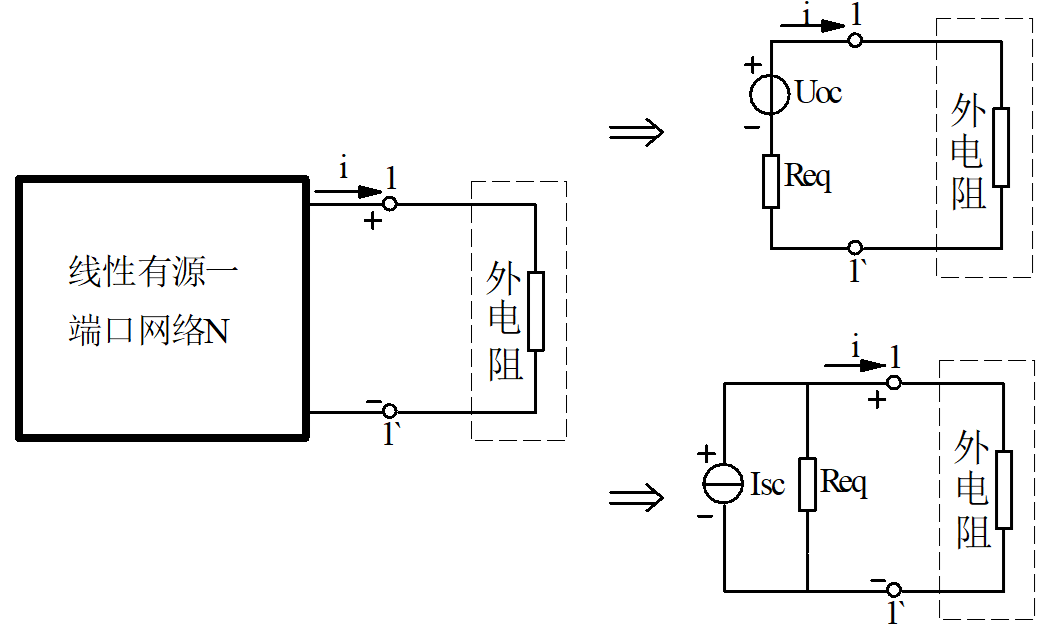
\includegraphics[width=0.6\textwidth]{graph1.png}
			\caption{一端口网络的等效置换}
			\label{fig:graph1}
		\end{figure}
	
	
	% 实验前思考题
	\subsection{实验预习题}
	
	% 思考题1
	\begin{question}
		用开路电压、短路电流法测量等效电阻时,开路电压、短路电流是否可以同时进行测量,为什么?
	\end{question}
	
	在使用开路电压和短路电流法测量电路的等效电阻时,实际操作中开路电压和短路电流是不能同时进行测量的。原因在于这两种测量方式的条件和对电路的影响完全不同。
	
	\textbf{开路电压测量}:在进行开路电压的测量时,测量对象(如一个电路或电池)的两端不接任何外部负载,即电路是开路状态。这种测量方式的目的是测定在无负载条件下电源的电压,即电源的最大电动势。在这种状态下,电路中的电流为零,因此不会有电流通过被测电源或电路,可以获得一个准确的开路电压值。
	
	\textbf{短路电流测量}:而在进行短路电流的测量时,测量对象的两端被直接短路,通过一个极低的电阻(接近于零),目的是测量在这种极端条件下通过电路的电流大小。这种状态下电路的电阻最小,电流达到最大值。这样做可以确定电源或电路在最大负载条件下的输出电流能力。
	
	由于开路状态下电路的电流为零,而短路状态下电流达到最大,这两种状态下的电路条件截然不同,因此不能同时进行测量。同时,若尝试同时进行这两种测量,可能会导致测量结果不准确,甚至损坏测量设备或被测电路。通常,在实际应用中,先后分别进行这两种测量,然后通过欧姆定律(V=IR)计算出等效电阻值,即使用开路电压除以短路电流的方法得到等效电阻值:$ R_{\text{等效}} = \dfrac{V_{\text{开路}}}{I_{\text{短路}}} $。这种方法适用于简单电路的等效电阻测量,尤其是在需要估计电源内阻或某些电气元件的等效电阻时非常有效。
	

%	开路电压和短路电流一般不可以同时进行测量,因为它们是针对同一个网络的两种测量方法,而在实际测量中很难同时实现。在实际测量过程中,需要对网络进行两种不同的激励:开路电压测量需要断开电路使得电流为零,而短路电流测量需要将电路短接使得电压为零。因此,在同一时刻只能选择一种测量方法进行。


	% % 思考题2
	% \begin{question}
		
	% \end{question}
	
	% % 思考题3
	% \begin{question}
		
	% \end{question}
	
	% ---
	
	
	
	% 实验记录	
	\clearpage
	
	% 顶栏
	\begin{table}
		\renewcommand\arraystretch{1.7}
		\centering
		\begin{tabularx}{\textwidth}{|X|X|X|X|}
			\hline
			专业: & 物理学 & 年级: & 2022级 \\
			\hline
			姓名: & 戴鹏辉、杨舒云 & 学号: & 22344016、22344020\\
			\hline
			室温: & 23\degree C & 实验地点: & A522 \\
			\hline
			学生签名:& 见\textbf{附件}部分 & 评分: &\\
			\hline
			实验时间:& 2024/3/18 & 教师签名:&\\
			\hline
		\end{tabularx}
	\end{table}
	% ---
	
	% 小标题
	\section{ET1-4 戴维南定理和诺顿定理  \quad\heiti 实验记录}
	% ---
	
	% 实验过程记录
	\subsection{实验内容、步骤与结果}
	
	%
	\subsubsection{操作步骤记录}
	
	实验用有源一端口网络如\cref{fig:graph2}所示。
	

		\begin{figure}[htbp]
			\centering
			\subfloat[实验用有源一端口网络电路图]
			{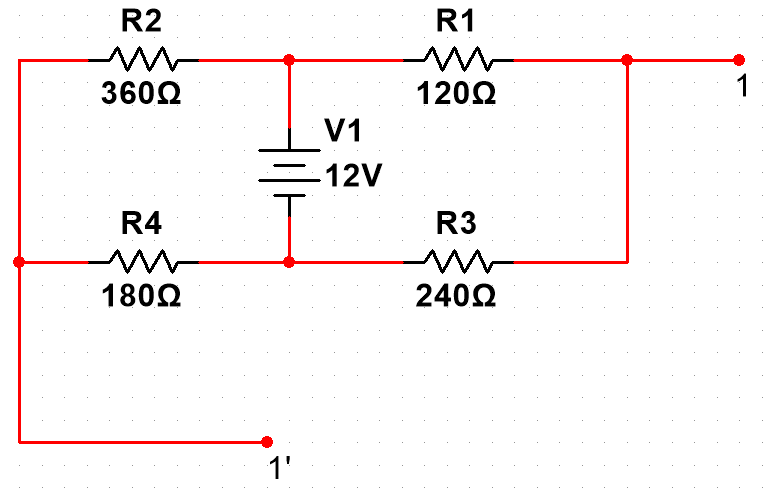
\includegraphics[width=0.4\textwidth]{graph2-1.png}\label{fig:graph2-1}}
			\quad
			\subfloat[实验用有源一端口网络实物图]
			{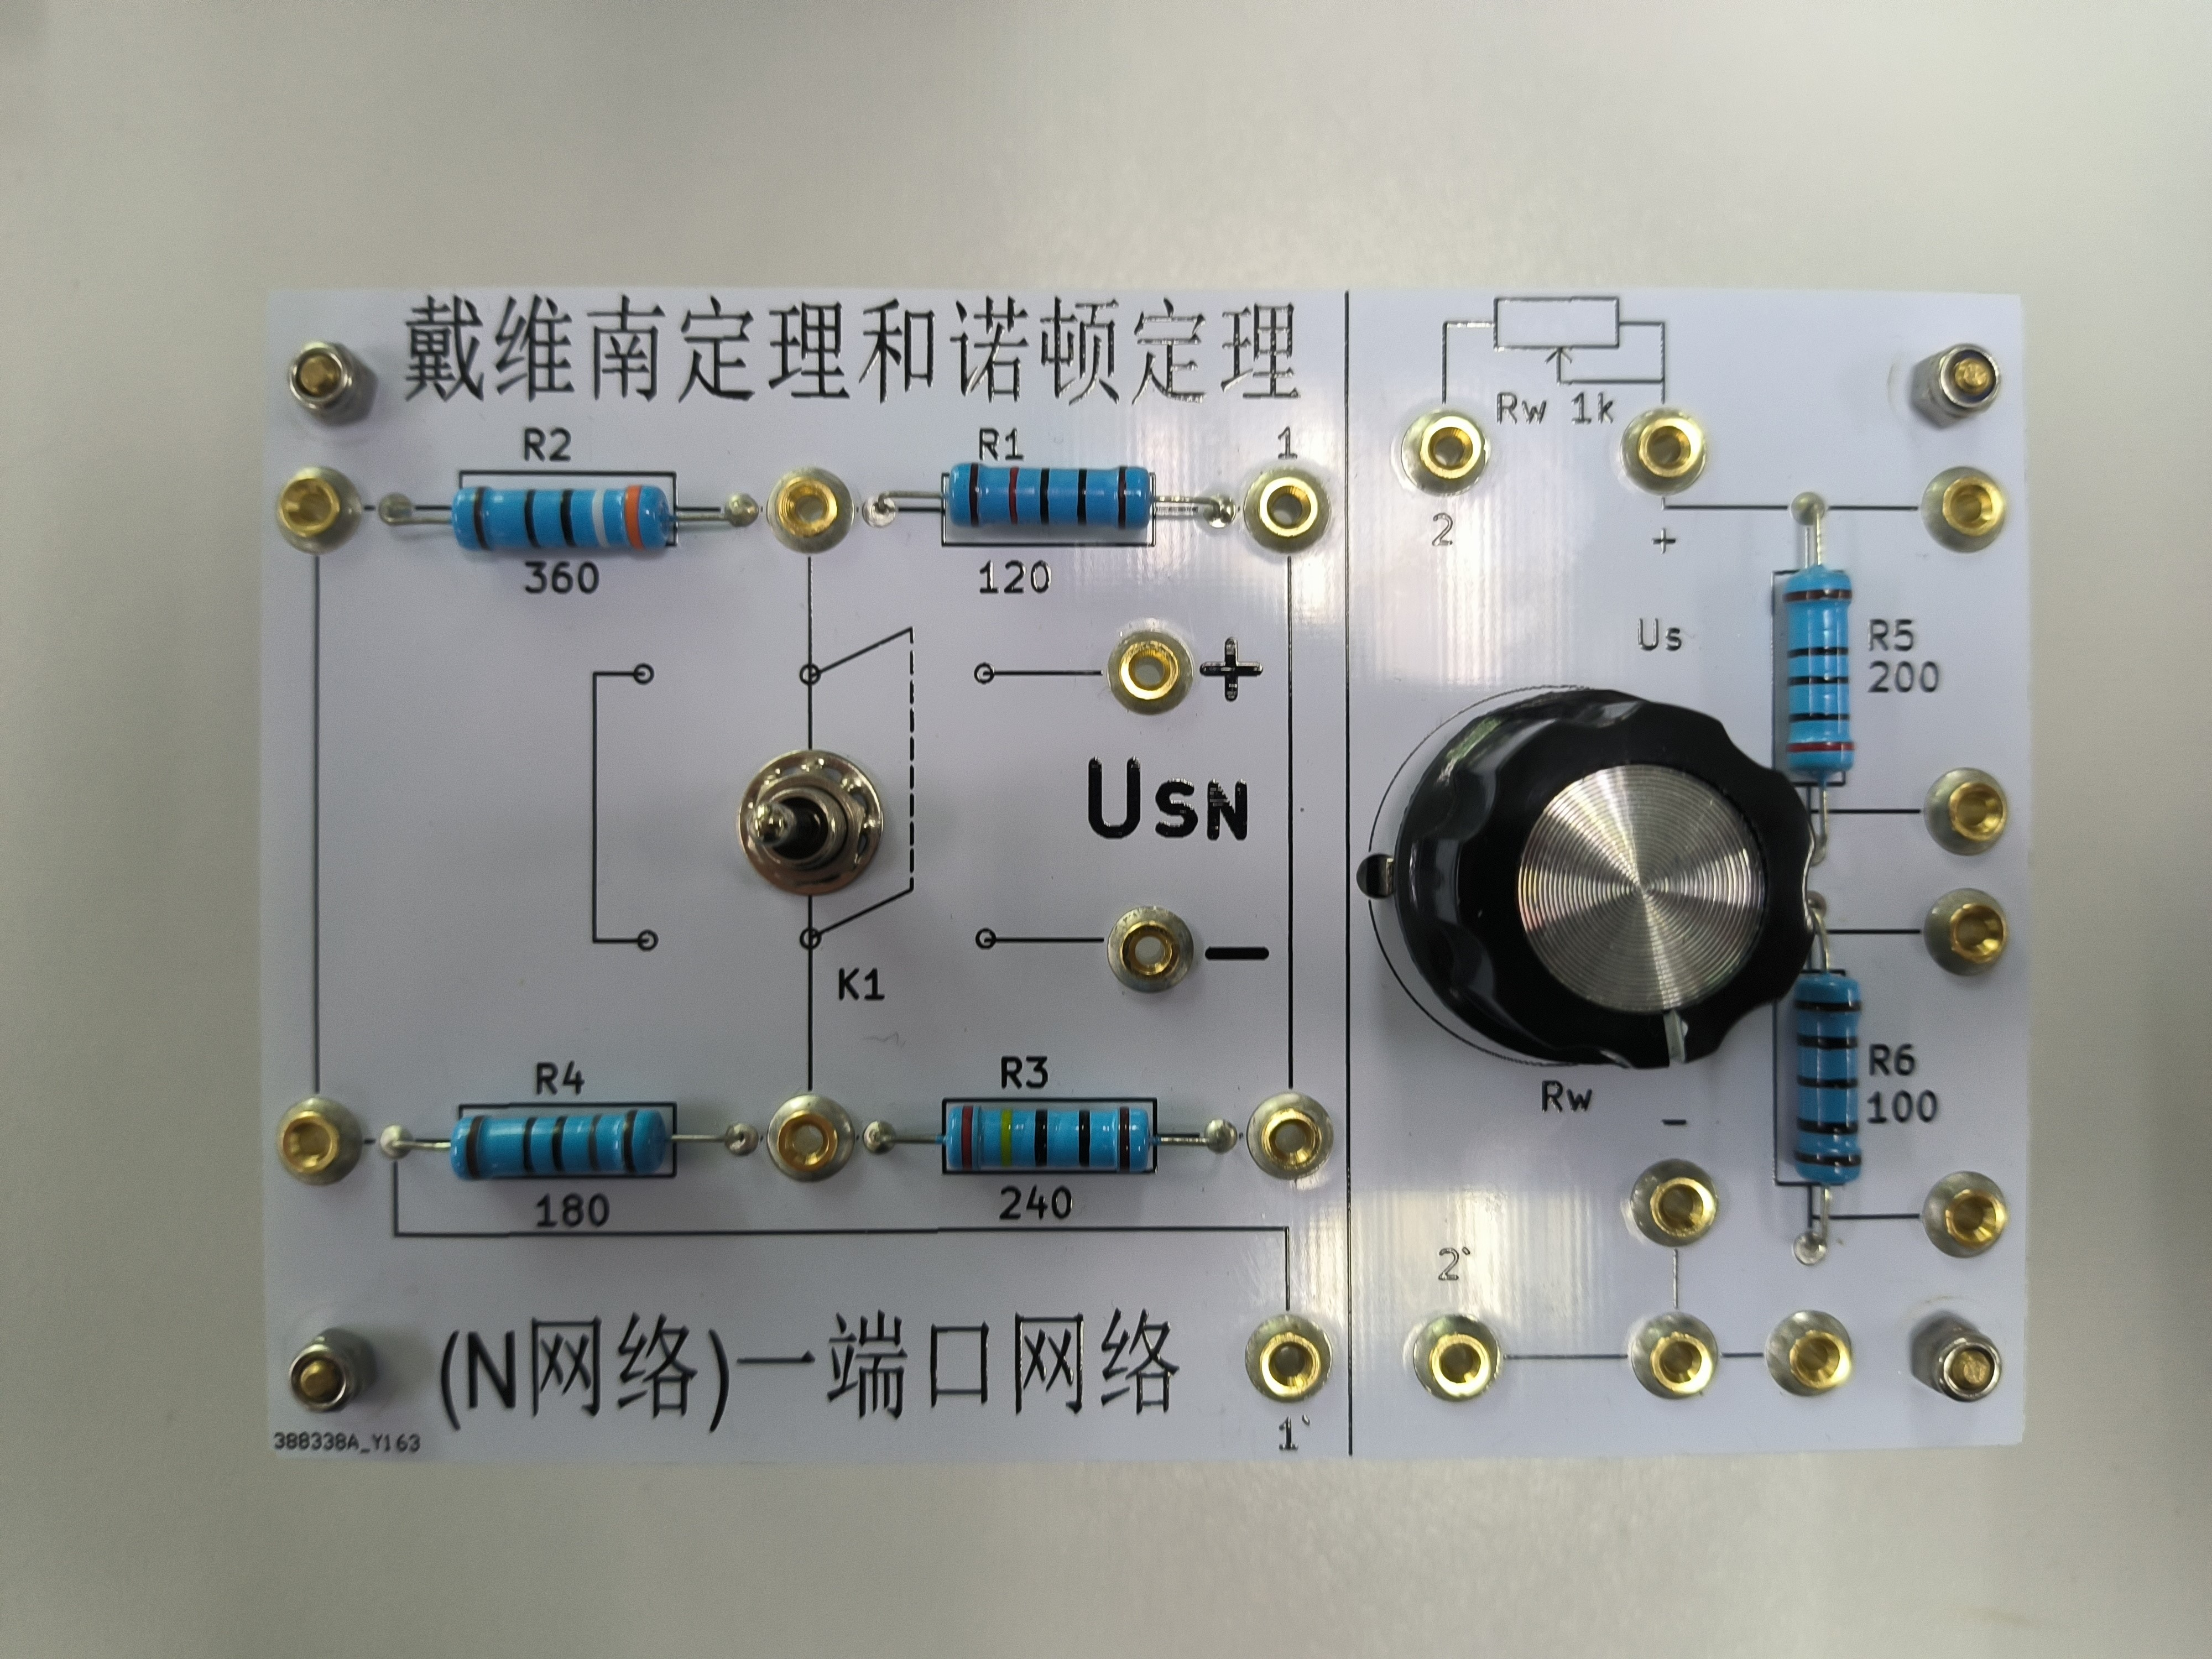
\includegraphics[width=0.4\textwidth]{graph2-2.jpg}\label{fig:graph2-2}}
			\quad
			\caption{实验用线性一端口网络}
			\label{fig:graph2}
		\end{figure}


	% \begin{figure}[htbp]
	% 	\centering
	% 	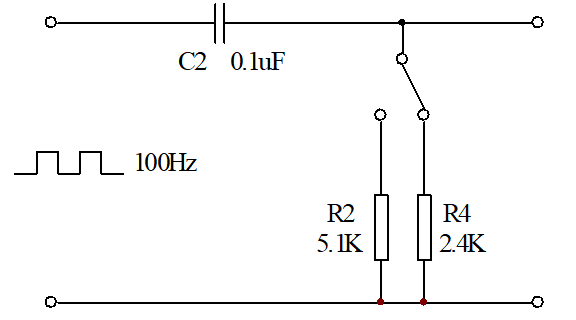
\includegraphics[width=0.6\textwidth]{graph2.png}
	% 	\caption{实验用有源一端口网络}
	% 	\label{fig:graph2}
	% \end{figure}
	
	\begin{enumerate}
		\item 直接测量有源一端口网络的开路电压$U_{OC}$、短路电流$I_{SC}$:在有源二端网络输出端开路时,用电压表直接测其输出端的开路电压$U_{oc}$,然后再将其输出端短路,用电流表测其短路电流$I_{sc}$。
		

		\begin{figure}[htbp]
			\centering
			\subfloat[开路电压、短路电流法]
			{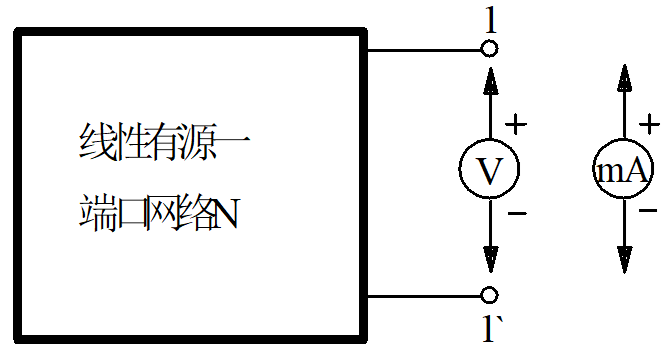
\includegraphics[width=0.35\textwidth]{graph1-1.png}\label{fig:graph1-1}}
			\quad
			\subfloat[电压零示法、电流零示法]
			{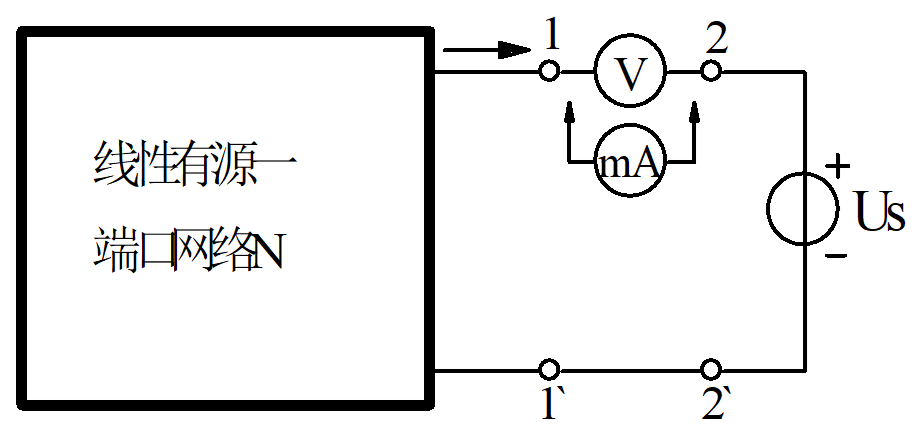
\includegraphics[width=0.35\textwidth]{graph1-2.png}\label{fig:graph1-2}}
			\quad
			% \caption{慧差实验结果图}
			\label{fig:graph10}
		\end{figure}

		% \begin{figure}[htbp]
		% 	\centering
		% 	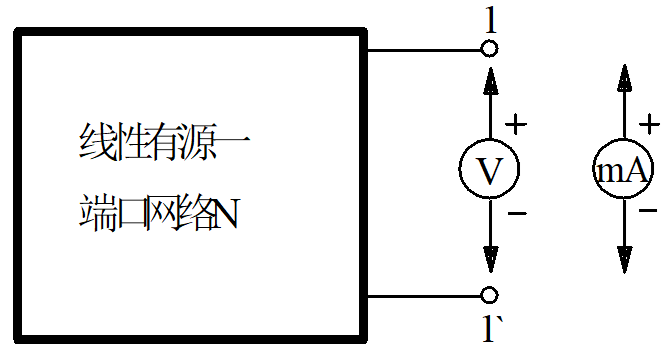
\includegraphics[width=0.6\textwidth]{graph1-1.png}
		% 	\caption{开路电压、短路电流法}
		% 	\label{fig:graph1-1}
		% \end{figure}

		\item 测量有源一端口网络的开路电压$U_{OC}$
		\begin{enumerate}
			\item 电压零示法:在测量具有高内阻有源二端网络的开路电压时,用电压表直接测量会造成较大的误差。为了消除电压表内阻的影响,往往采用零示测量法,零示法测量原理是用一低内阻的稳压电源与被测有源二端网络进行比较,当稳压电源的输出电压与有源二端网络的开路电压相等时,电压表的读数将为“0”。然后将电路断开,测量此时稳压电源的输出电压,即为被测有源二端网络的开路电压。

			\item 电流零示法:用电流表或检流计判断等电位的方法,条件与方法同上,测量结果较为精确,但也与电流表灵敏度有关。
		\end{enumerate}
		
		% \begin{figure}[htbp]
		% 	\centering
		% 	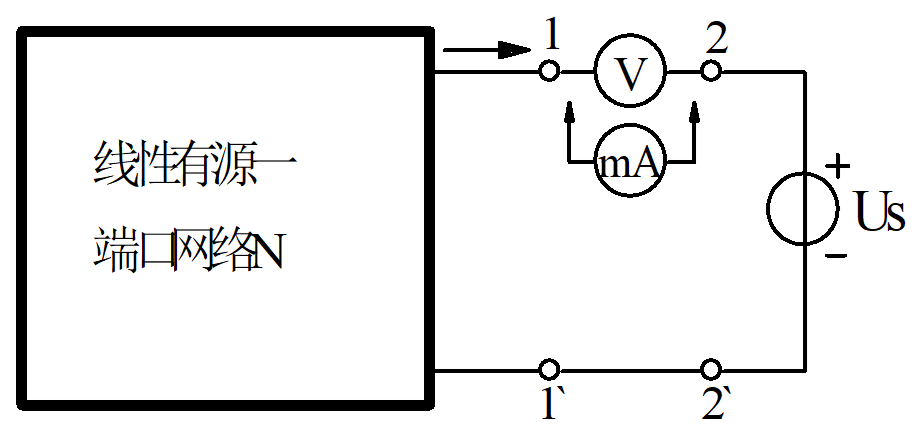
\includegraphics[width=0.6\textwidth]{graph1-2.png}
		% 	\caption{电压零示法、电流零示法}
		% 	\label{fig:graph1-2}
		% \end{figure}

		\item 测量有源一端口网络的等效电阻$R_{eq}$
		\begin{enumerate}
			\item 开路电压、短路电流法:在有源二端网络输出端开路时,用电压表直接测其输出端的开路电压$U_{oc}$,然后再将其输出端短路,用电流表测其短路电流$I_{sc}$(这一步可以直接利用第一个步骤所测得的数据),则等效内阻为$R_{eq}=\frac{U_{oc}}{I_{sc}}$。如果二端网络的内阻很小,若将其输出端口短路则易损坏其内部元件,不宜用此法。
			\item 伏安法:当一端口网络内部无源时,整个一端口网络可看成一个电阻。
			
			\begin{figure}[htbp]
				\centering
				\subfloat[伏安法]
				{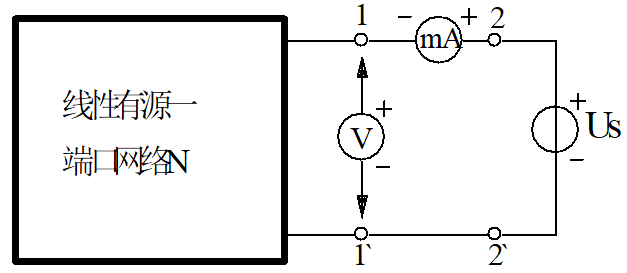
\includegraphics[width=0.35\textwidth]{graph1-3.png}\label{fig:graph1-4}}
				\quad
				\subfloat[半流法]
				{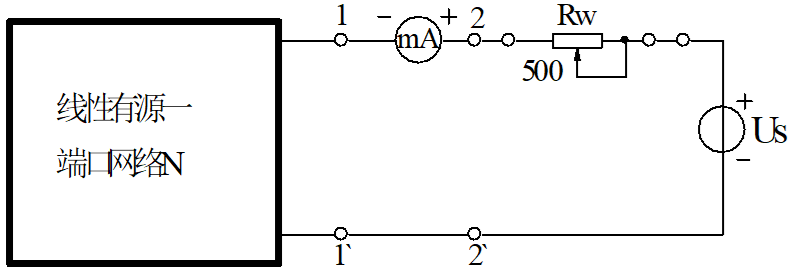
\includegraphics[width=0.35\textwidth]{graph1-4.png}\label{fig:graph1-4}}
				\quad
				% \caption{慧差实验结果图}
				\label{fig:graph1-5}
			\end{figure}

			% \begin{figure}[htbp]
			% 	\centering
			% 	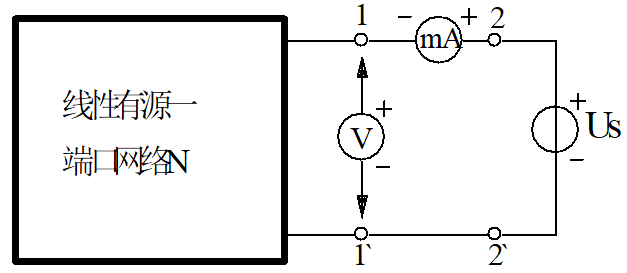
\includegraphics[width=0.6\textwidth]{graph1-3.png}
			% 	\caption{伏安法}
			% 	\label{fig:graph1-3}
			% \end{figure}
			
			\textbf{事实上,真正的伏安法应当是“测电源的伏安法”:伏安法测 \( R_{eq} \) 用电压表、电流表测出有源二端网络的外特性曲线,根据外特性曲线求出斜率 \( \tan \phi \),则内阻也可以先测量开路电压 \( U_{oc} \),再测量电流为额定值 \( I_N \) 时的输出端电压值 \( U_N \)。}
			
			\item 半流法:当调$R_W$使电流表指示为伏安法时电流表的指示的一半时,此时电位器$R_W$的值等于一端口网络等效电阻$R_{eq}$,断开电流表和外加电源,测$R_W$值就等于是$R_{eq}$。
			
			% \begin{figure}[htbp]
			% 	\centering
			% 	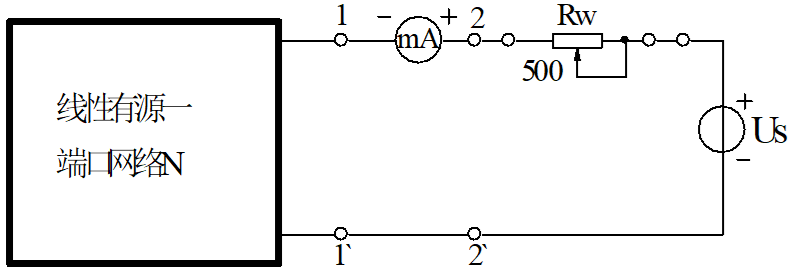
\includegraphics[width=0.6\textwidth]{graph1-4.png}
			% 	\caption{半流法}
			% 	\label{fig:graph1-4}
			% \end{figure}

			\item 半压法:半电压法测$R_{eq}$当负载电压为被测网络开路电压的一半时,负载电阻(由电阻箱的读数确定)即为被测有源二端网络的等效内阻值。
			
			\begin{figure}[htbp]
				\centering
				\subfloat[半压法]
				{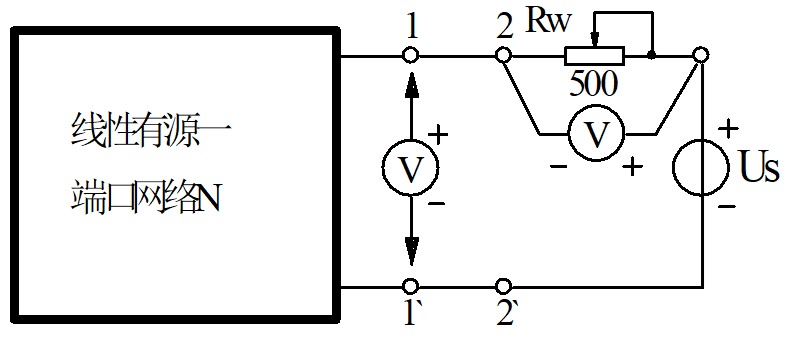
\includegraphics[width=0.3\textwidth]{graph1-5.png}\label{fig:graph1-5}}
				\quad
				\subfloat[直接测量法]
				{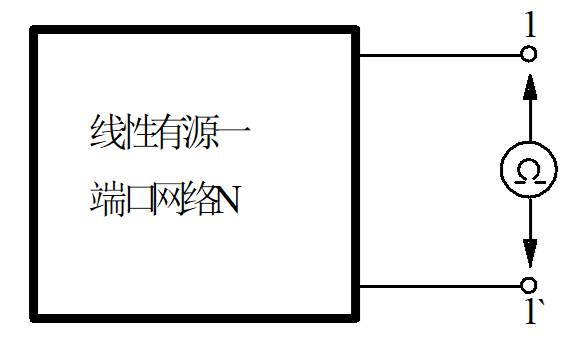
\includegraphics[width=0.3\textwidth]{graph1-6.png}\label{fig:graph1-6}}
				\quad
				% \caption{慧差实验结果图}
				\label{fig:graph1-5}
			\end{figure}

			% \begin{figure}[htbp]
			% 	\centering
			% 	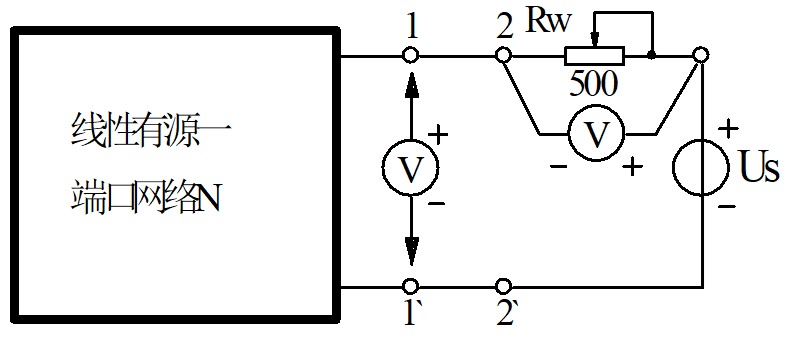
\includegraphics[width=0.6\textwidth]{graph1-5.png}
			% 	\caption{半压法}
			% 	\label{fig:graph1-5}
			% \end{figure}

			\item 欧姆表直接测量法:当一端口网络内部无源时,可用万用表欧姆档测量或直流电桥直接测量两端电阻(此种方法只适用于中值、纯电阻电路)。
			
						
			% \begin{figure}[htbp]
			% 	\centering
			% 	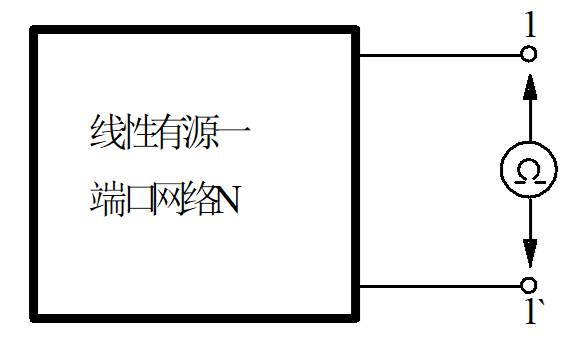
\includegraphics[width=0.6\textwidth]{graph1-6.png}
			% 	\caption{直接测量法}
			% 	\label{fig:graph1-6}
			% \end{figure}

		\end{enumerate}

		\begin{figure}[htbp]
			\centering
			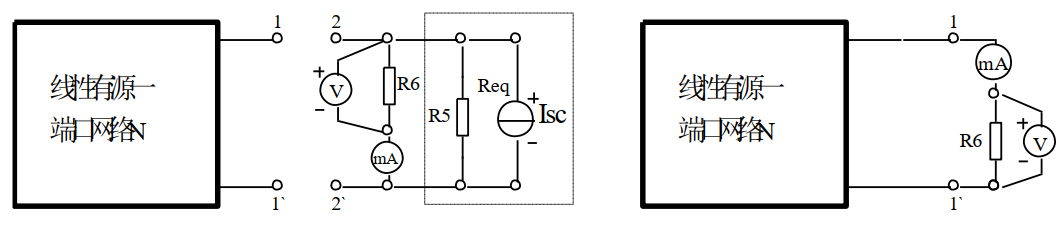
\includegraphics[width=0.9\textwidth]{graph1-7.png}
			\caption{验证戴维南定理和诺顿定理电路图}
			\label{fig:graph1-7}
		\end{figure}

		\item 验证戴维南定理
			\begin{enumerate}
				\item 戴维南等效电路外接负载。首先组成一个戴维南等效电路,即用外电源$U_S$与戴维南等效电阻$R_5=R_{eq}$相串后,外接$R_6=100\Omega$的负载,然后测电阻$R_6$两端电压$U_{R_6}$和流过$R_6$的电流值$I_{R_6}$。
				
				\item N有源网络1-1’端口外接负载。同样接$R_6=100\Omega$的负载,测电压$U_{R_6}$与电流$I_{R_6}$。将测试结果与上一步作比较,验证戴维南定理。
			\end{enumerate}


		\item 验证诺顿定理
			\begin{enumerate}
				\item 诺顿等效电路外接负载。首先组成一个诺顿等效电路,即用外加电流源$I_S$与戴维南等效电阻$R_5=R_{eq}$相并后,外接$R_6=100\Omega$的负载,然后测电阻$R_6$两端电压$U_{R_6}$和流过$R_6$的电流值$I_{R_6}$。
				\item 与上面测试结果进行比较,验证诺顿定理
			\end{enumerate}


		\item 利用函数信号发生器验证戴维南定理
			\begin{enumerate}
				\item 关于开路电压、短路电流法
				
				讲义指出:测量内阻时不能采用直接法,即输出不能直接短路,否则函数发生器有危险,出现过流保护,测量不对,因此要采用其他的方法测量内阻!
				
				这里的直接法便是开路电压、短路电流法,这种方法不能用于测量函数信号发生器。
				
				\item 关于伏安法、半压半流法和欧姆表直接测量法
				
				接着,我们考虑了将偏置设置为零然后外接电源利用伏安法、半压半流法和欧姆表直接测量法,然而该信号发生器生产厂商的技术客服告诉我,不能对信号发生器倒灌电流,这可能会导致信号发生器损坏。
				
				\item 利用前面提出的“测电源的伏安法”
				
				最后,我们在讨论与思考后选择了前面提出的“测电源的伏安法”,\cref{fig:graph5}中虚线框内为信号发生器,$R_0$即为信号发生器内阻,$R_1=100\Omega$为电路保护电阻。通过改变外负载$R_x$的电阻值,记录$R_x$两端电压和通过其的电流,得到信号发生器的外输出特性曲线,其中纵轴截距即为信号发生器输出电压,斜率即为$-(R_0+R_x)$。
				
				\begin{figure}[htbp]
					\centering
					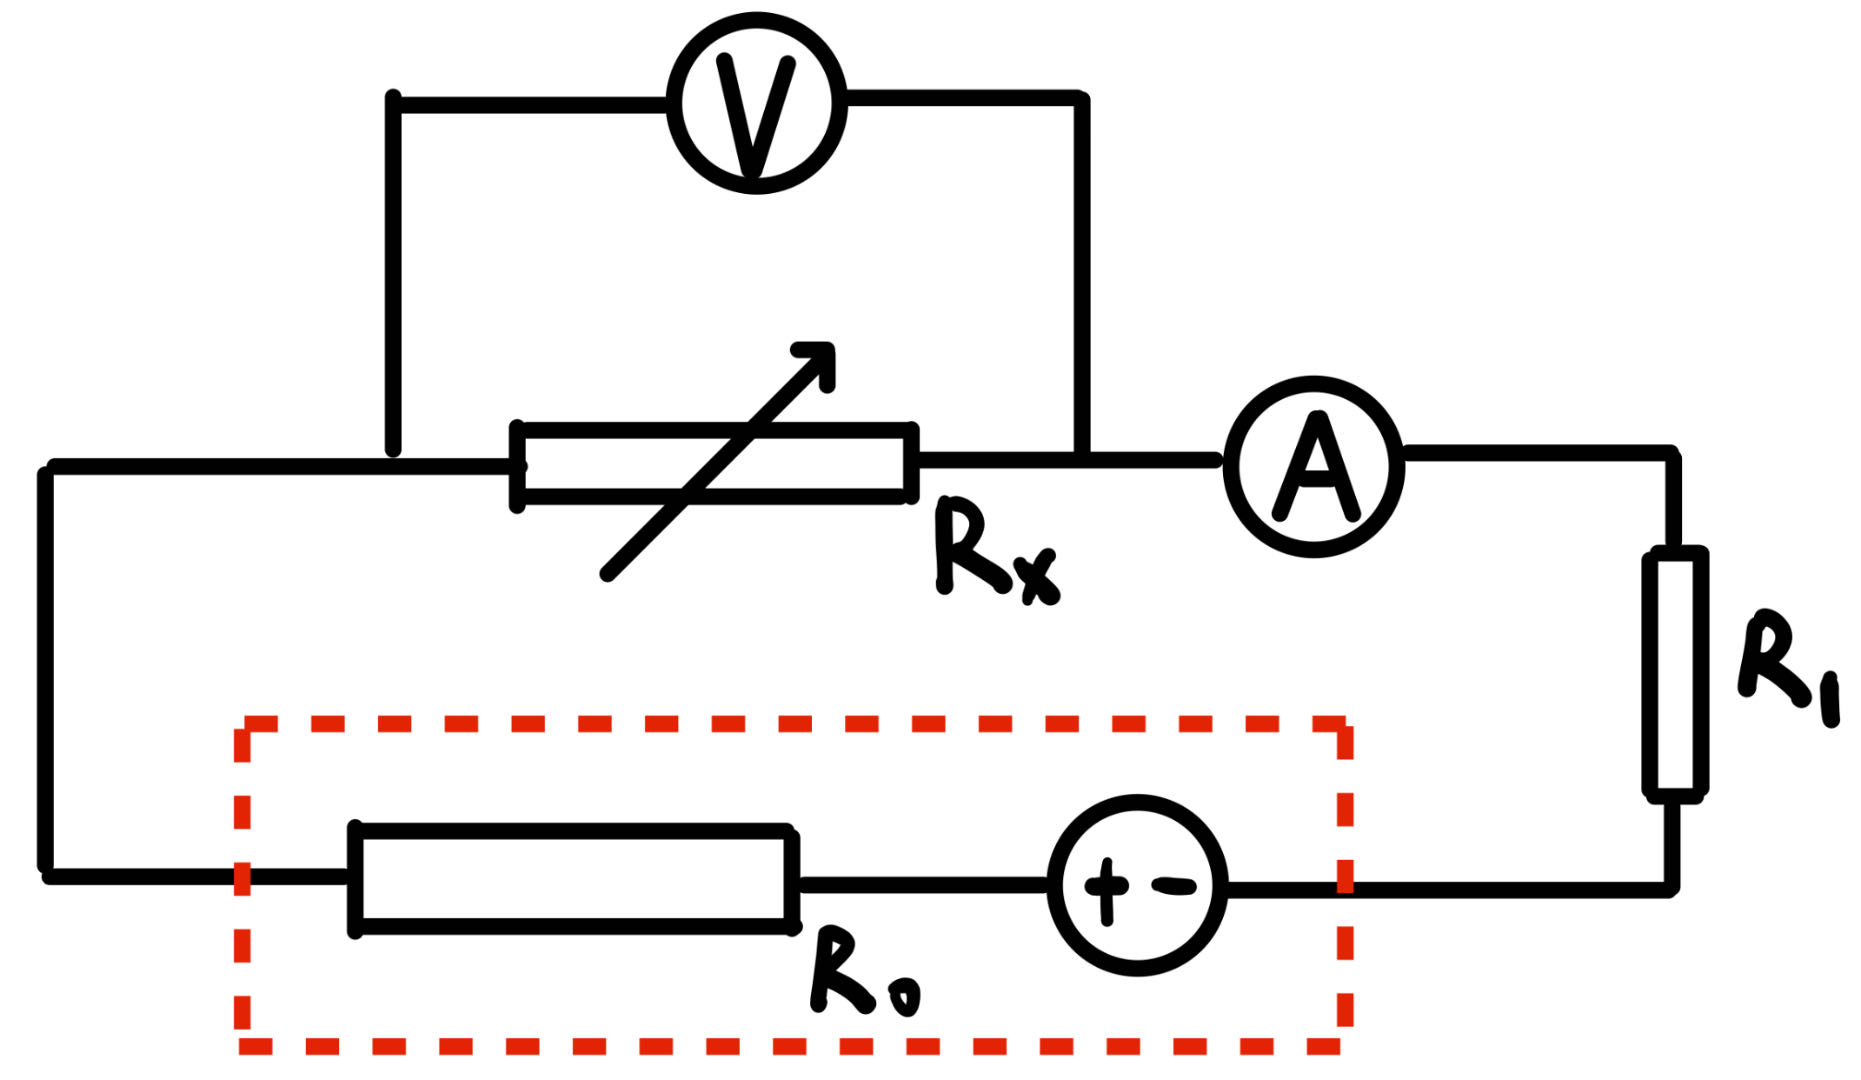
\includegraphics[width=0.4\textwidth]{graph5.jpg}
					\caption{利用函数信号发生器验证戴维南定理电路图}
					\label{fig:graph5}
				\end{figure}
																
			\end{enumerate}
	\end{enumerate}
	
	%
	\subsubsection{实验结果展示}
	\begin{enumerate}
		\item 直接测量有源一端口网络的开路电压$U_{OC}$、短路电流$I_{SC}$
		
		\textbf{直接测量}得到:$U_{OC}=3.965V$,$I_{SC}=19.900mA$。
		
		\item 测量有源一端口网络的开路电压$U_{OC}$
		
		利用\textbf{电压零示法},在电压表示数为零时,补偿电源设置为3.937V,测得$U_{OC}=3.914V$;
		
		利用\textbf{电流零示法},电流表示数接近零(由于精度问题无法调至零),测得$U_{OC}=3.913V$。
		
		\item 测量有源一端口网络的等效电阻$R_{eq}$
		
		根据\textbf{开路电压、短路电流法},由$U_{OC}=3.965V$,$I_{SC}=19.900mA$得到$R_{eq}=199.246\Omega$;
		
		而利用\textbf{伏安法},当提供(测量)电压为10V时,电流表示数为50.904mA,即测得$R_{eq}=196.46\Omega$,当提供(测量)电压为7V时,电流表示数为35.601mA,测得$R_{eq}=196.62\Omega$;
		
		对于\textbf{半流法},外加电源电压为10V,$I'_{SC}=25.452mA$时,测得$R_{eq}=193.0\Omega$;
		
		利用\textbf{半压法},外加电源电压为10V,$U_W=5V$时,测得$R_{eq}=193.5\Omega$;
		
		最后对于用\textbf{欧姆表直接测量},它的结果最接近理论值,测得$R_{eq}=200.1\Omega$。
		
		\item 验证戴维南定理和诺顿定理
		


			用线性端口网络供电时,得到$U_{R_6}=1.315V \quad I_{R_6}=13.302mA$\\
			用外置电压源供电时,得到$U_{R_6}=1.296V \quad I_{R_6}=13.050mA$\\
			用外置电流源供电时,得到$U_{R_6}=1.250V \quad I_{R_6}=12.900mA$\\

		\item 利用函数信号发生器验证戴维南定理
		


			测量结果如\cref{tab:tab2}所示。详见\textbf{数据分析}部分,在\cref{fig:graph6}中,$50\Omega$模式时,纵轴截距读出输出电压为9.80V,斜率读出等效内阻为152$\Omega$,扣去保护电阻后即得到信号发生器内阻约为52$\Omega$;$HighZ$模式时,纵轴截距读出输出电压为9.81V,斜率读出等效内阻为152$\Omega$,扣去保护电阻后即得到信号发生器内阻约为52$\Omega$。
			
			\begin{table}[htbp]
				\centering
				\caption{信号发生器外输出特性测量}
				\begin{tabular}{|c|c|c|c|}
					\hline
					\multicolumn{2}{|c|}{50Ω} & \multicolumn{2}{c|}{高阻} \\
					\hline
					U/V & I/mA & U/V & I/mA \\
					\hline
					0.017 & 64.000 & 8.580 & 8.583 \\
					1.006 & 57.200 & 8.000 & 11.800 \\
					2.020 & 52.400 & 7.000 & 18.110 \\
					3.018 & 44.660 & 6.000 & 25.090 \\
					4.009 & 38.160 & 5.000 & 31.720 \\
					5.000 & 30.600 & 4.005 & 38.400 \\
					6.060 & 24.200 & 3.010 & 43.870 \\
					7.010 & 18.220 & 2.002 & 51.120 \\
					8.010 & 11.200 & 1.010 & 58.120 \\
					8.640 & 8.647 & 0.024 & 64.580 \\
					\hline
				\end{tabular}%
				\label{tab:tab2}%
			\end{table}%		
	\end{enumerate}
	
	% ---
	
	% 原始数据
	%\clearpage
	\subsection{原始数据记录}
	实验记录本上的原始数据见\cref{fig:figdata-1}、\cref{fig:figdata-2}、\cref{fig:figdata-3}、\cref{fig:figdata-4}(签字)、\cref{fig:figdata-5}和\cref{fig:figdata-6}(签字)。

	\begin{figure}[htbp]
		\centering
		\subfloat[原始数据1]
		{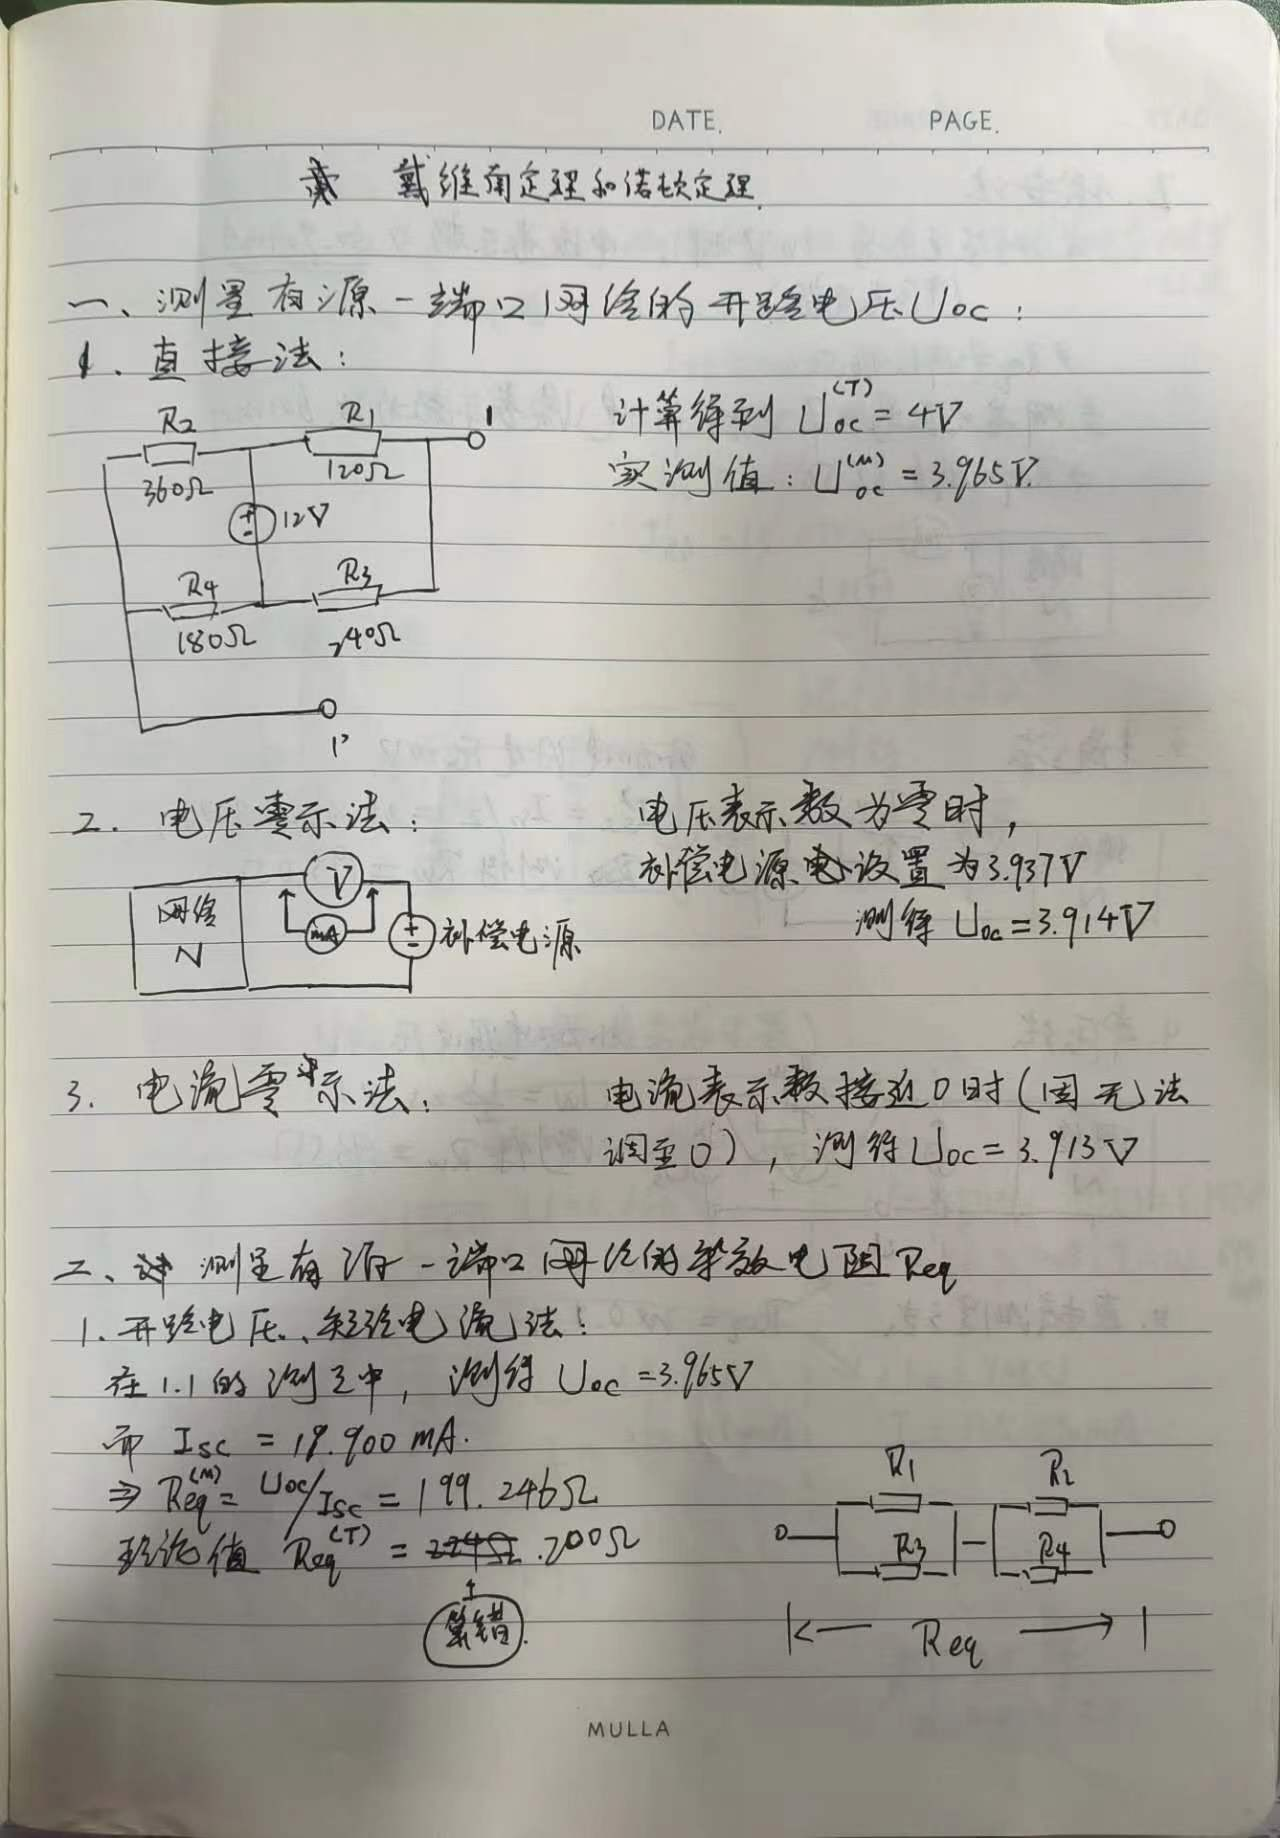
\includegraphics[width=0.28\textwidth]{ET1_4Gradata-1.jpg}\label{fig:figdata-1}}
		\quad
		\subfloat[原始数据2]
		{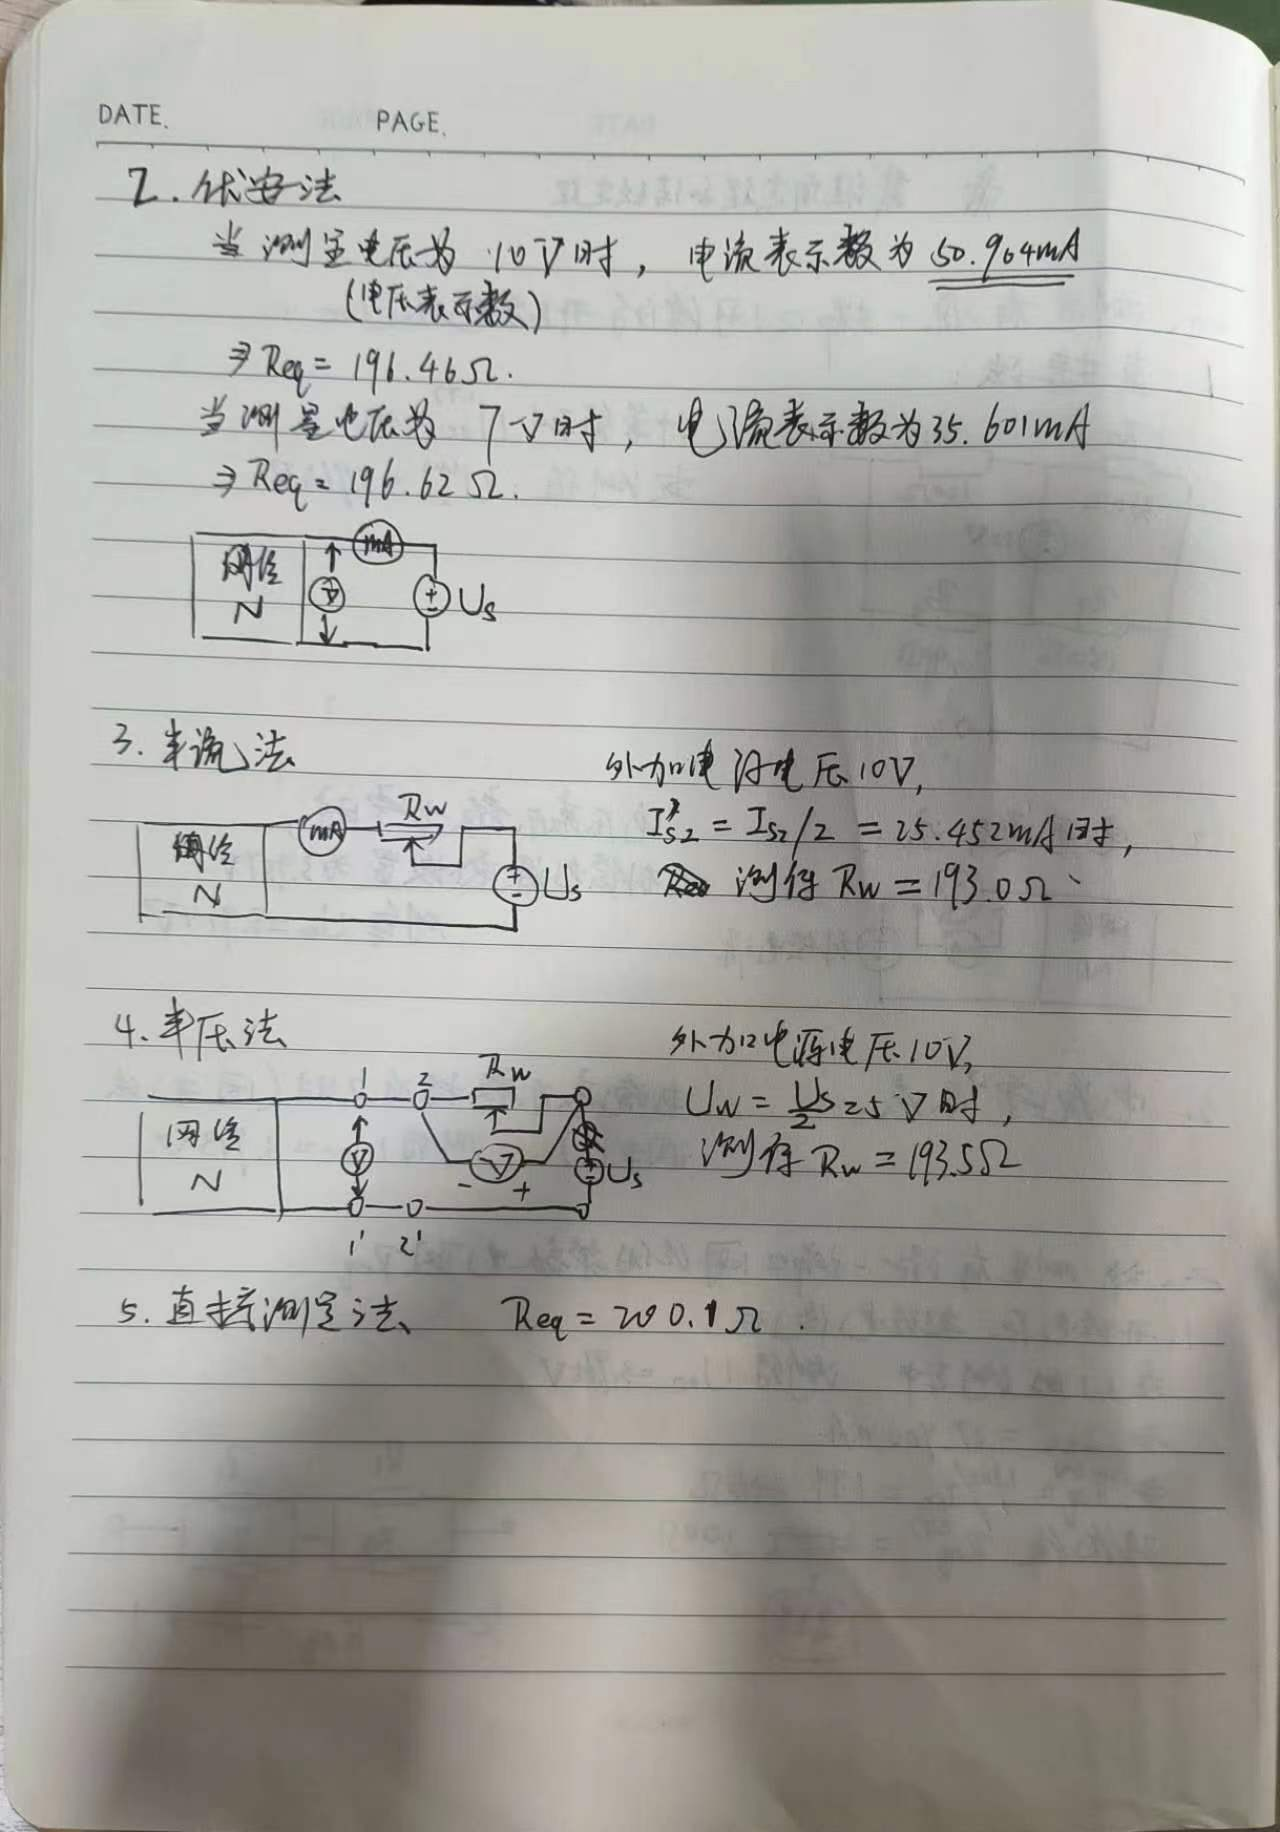
\includegraphics[width=0.28\textwidth]{ET1_4Gradata-2.jpg}\label{fig:figdata-2}}
		\quad
		\subfloat[原始数据3]
		{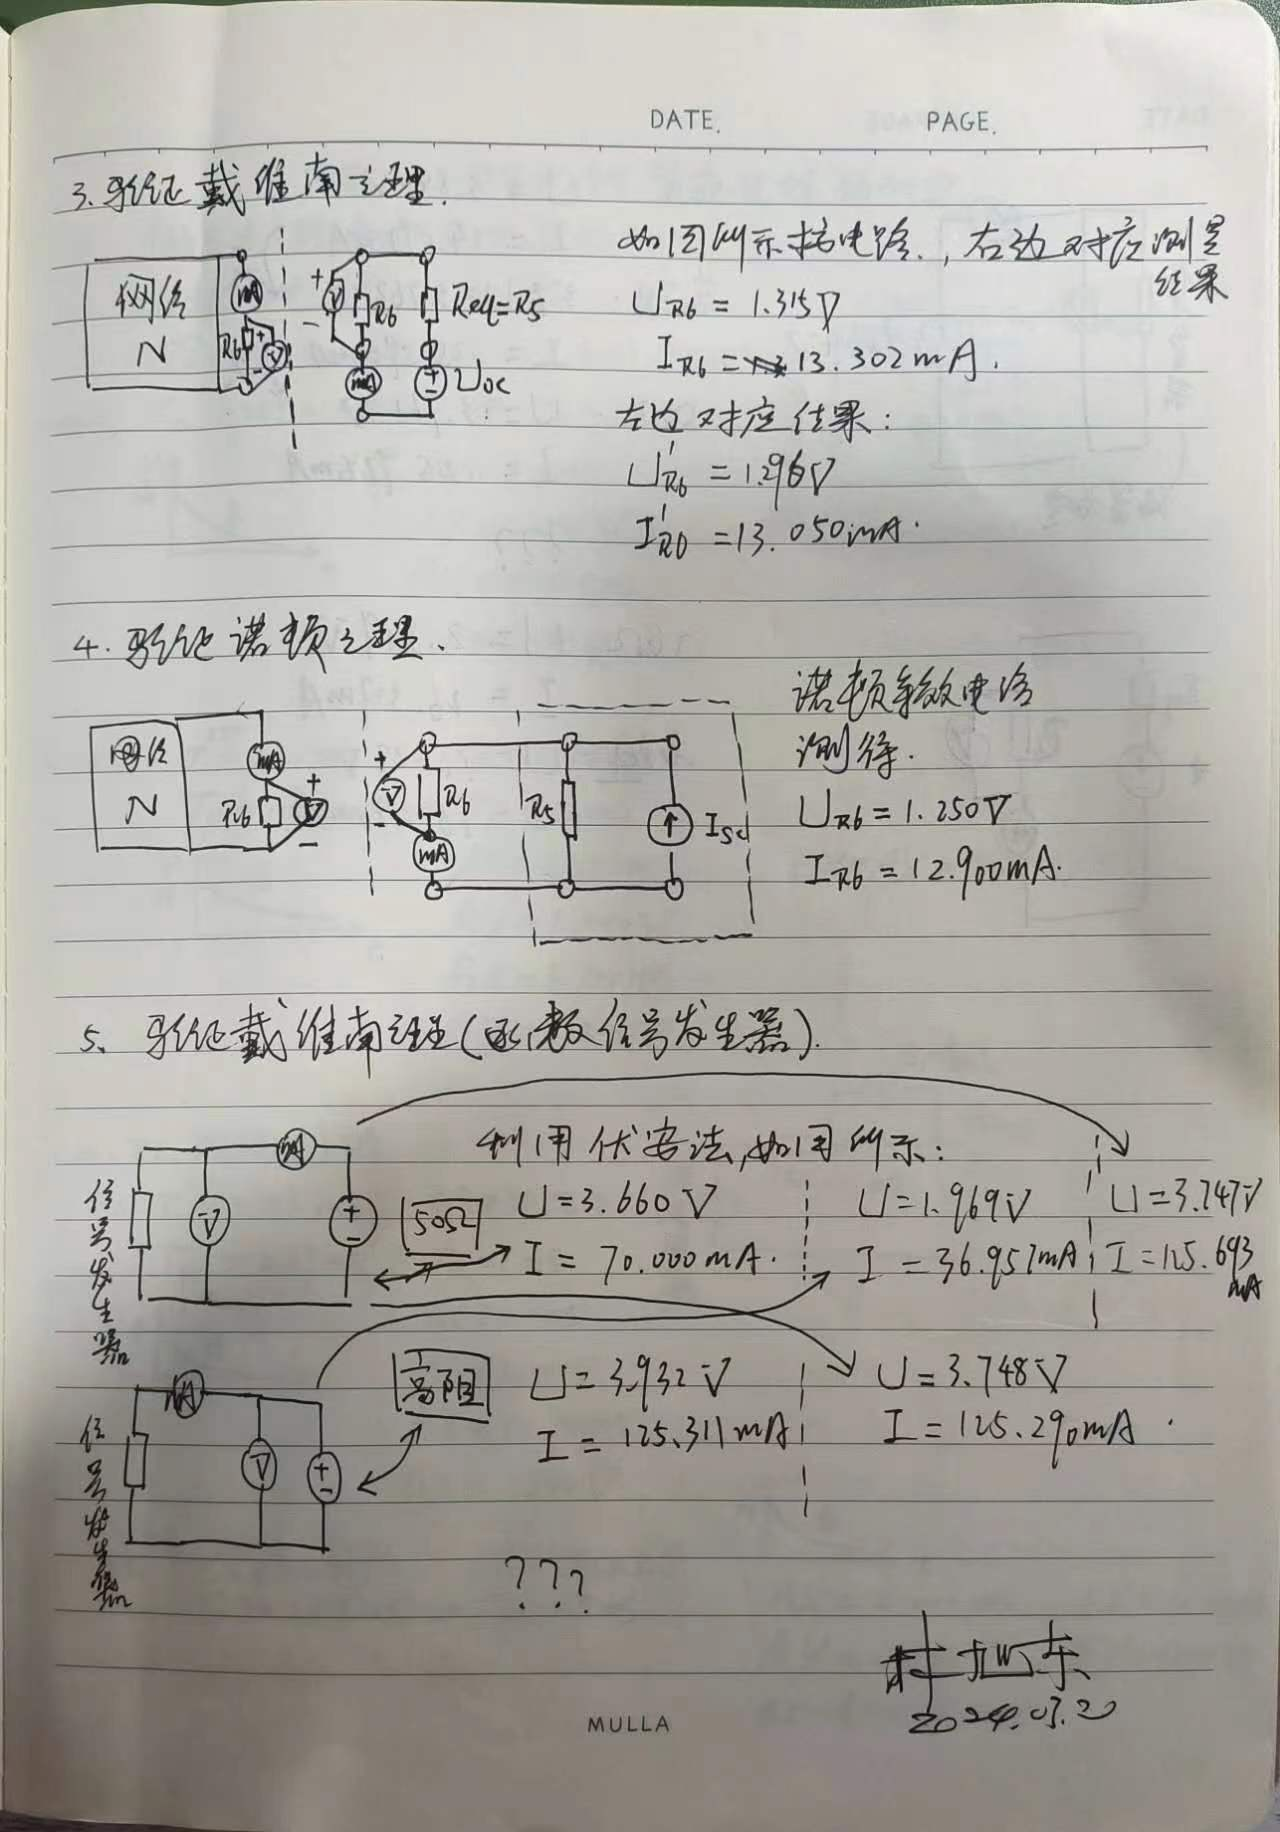
\includegraphics[width=0.28\textwidth]{ET1_4Gradata-3.jpg}\label{fig:figdata-3}}
		\quad
		\subfloat[原始数据4]
		{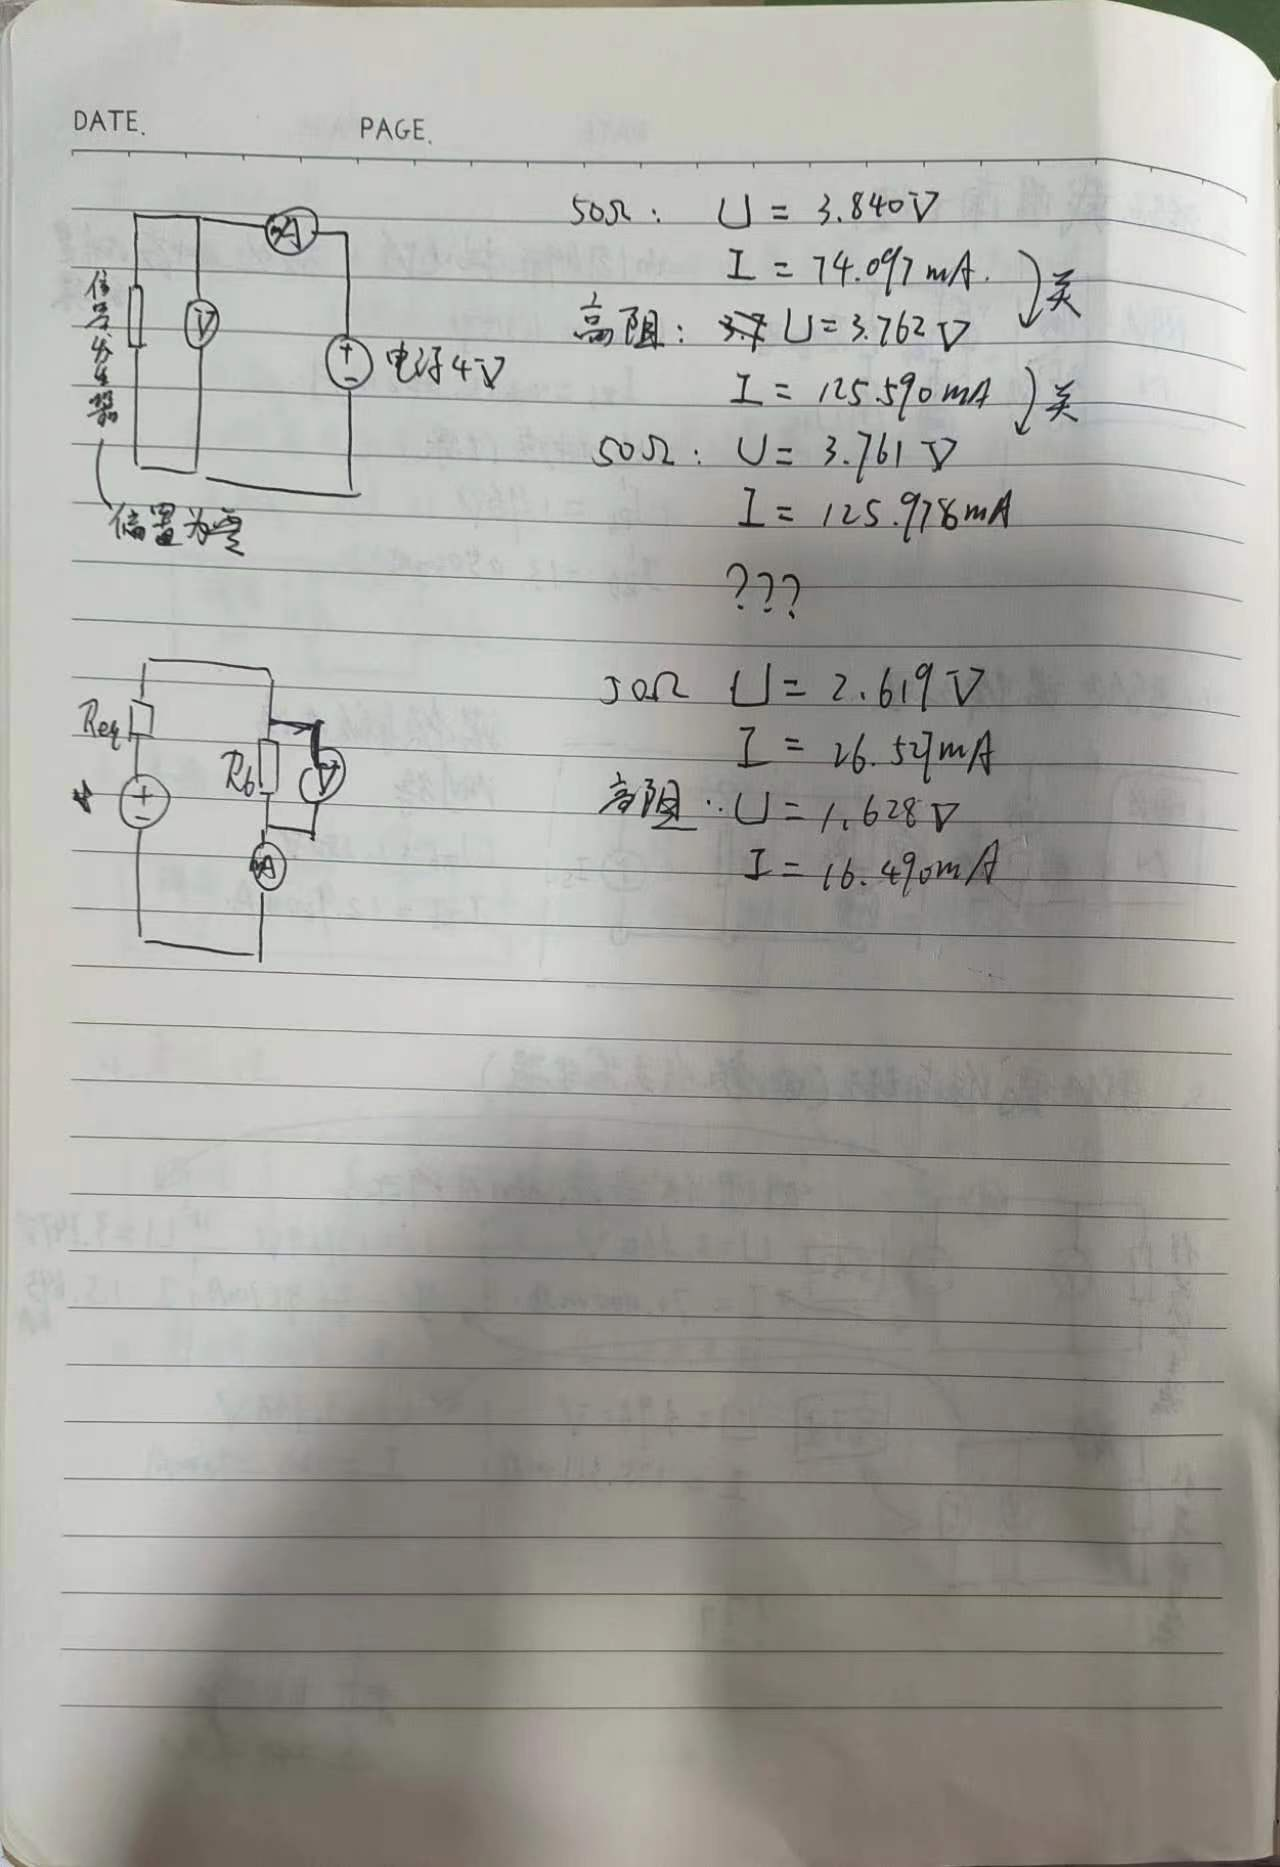
\includegraphics[width=0.28\textwidth]{ET1_4Gradata-4.jpg}\label{fig:figdata-4}}
		\quad
		\subfloat[原始数据5]
		{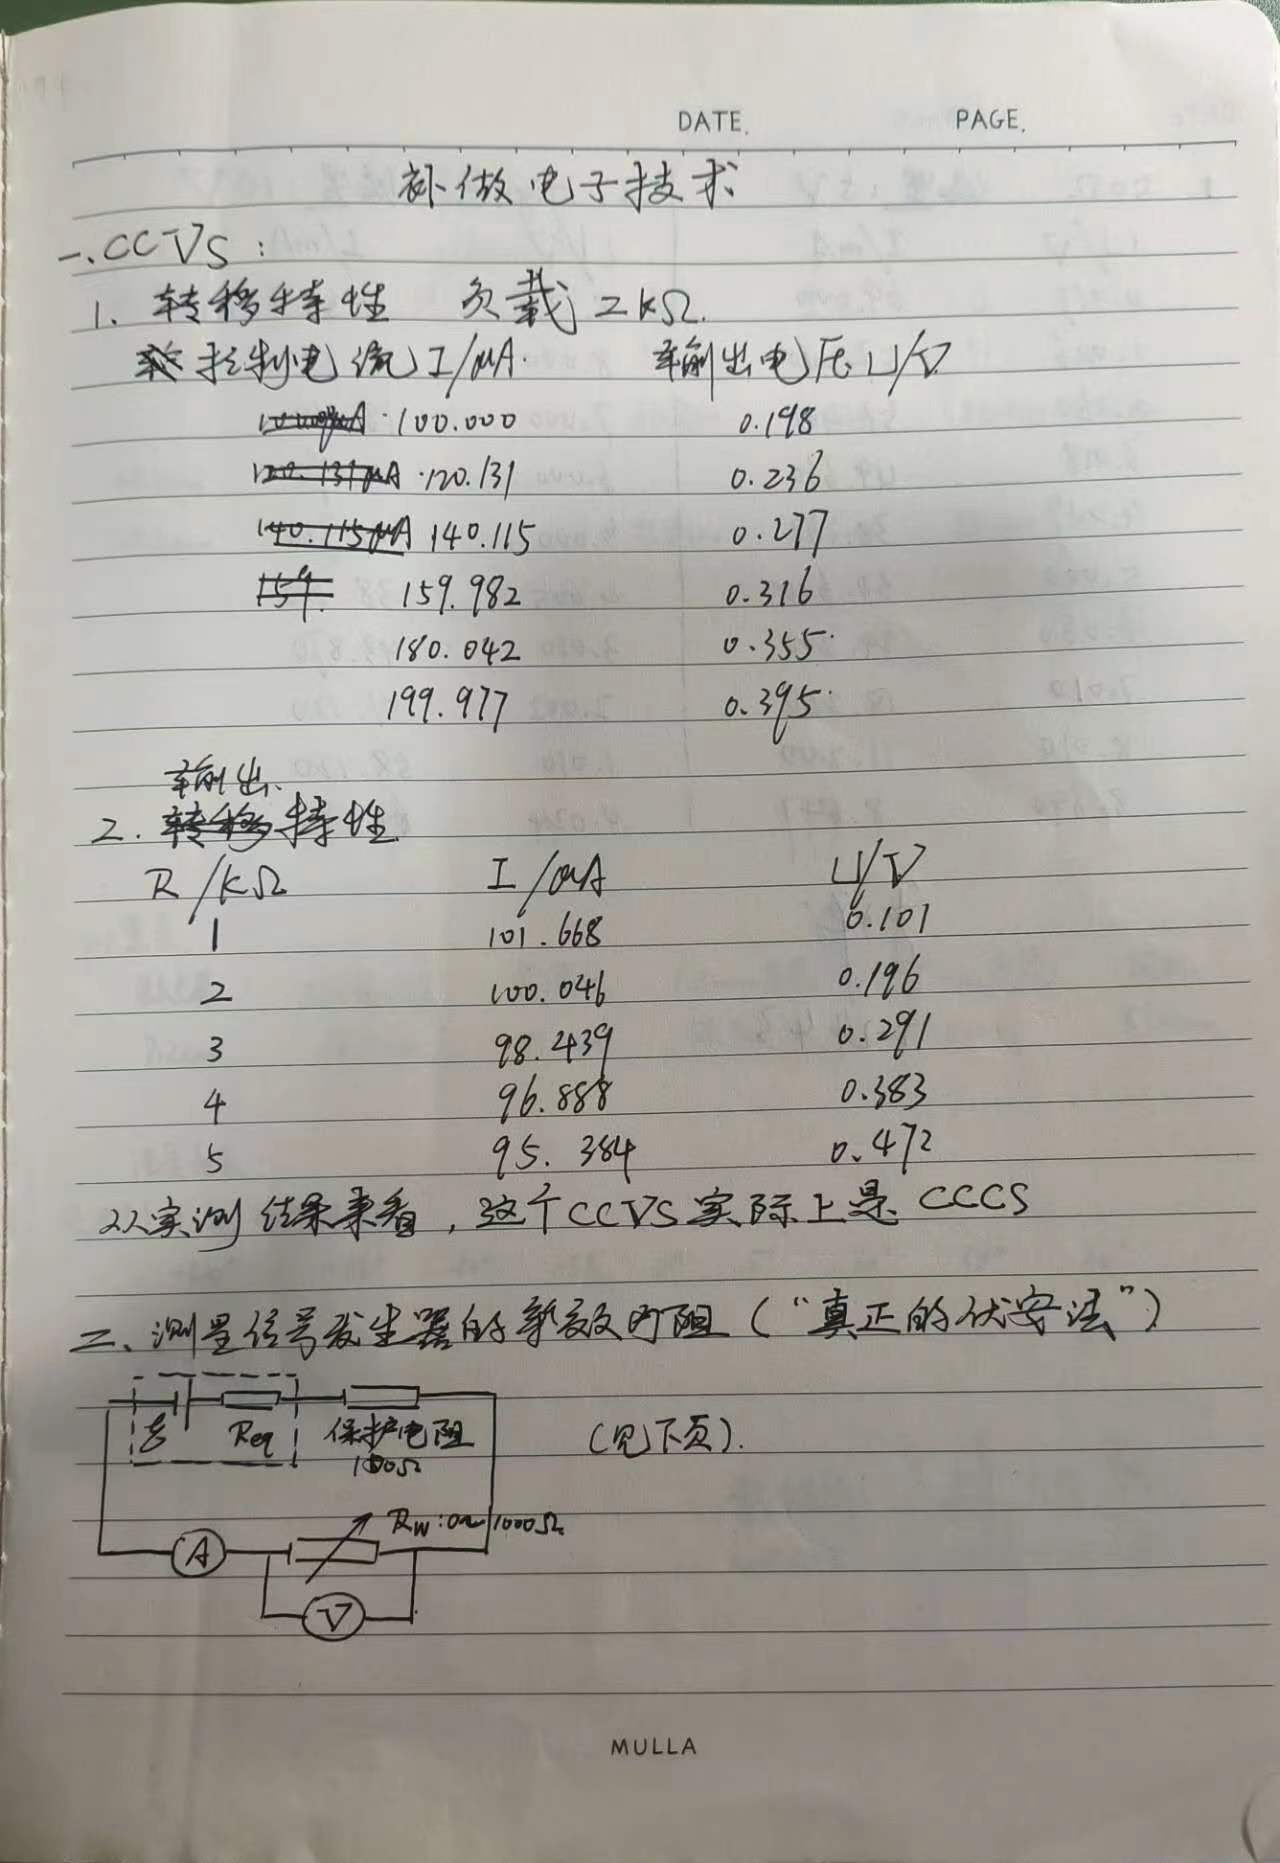
\includegraphics[width=0.28\textwidth]{ET1_4Gradata-5.jpg}\label{fig:figdata-5}}
		\quad
		\subfloat[原始数据6]
		{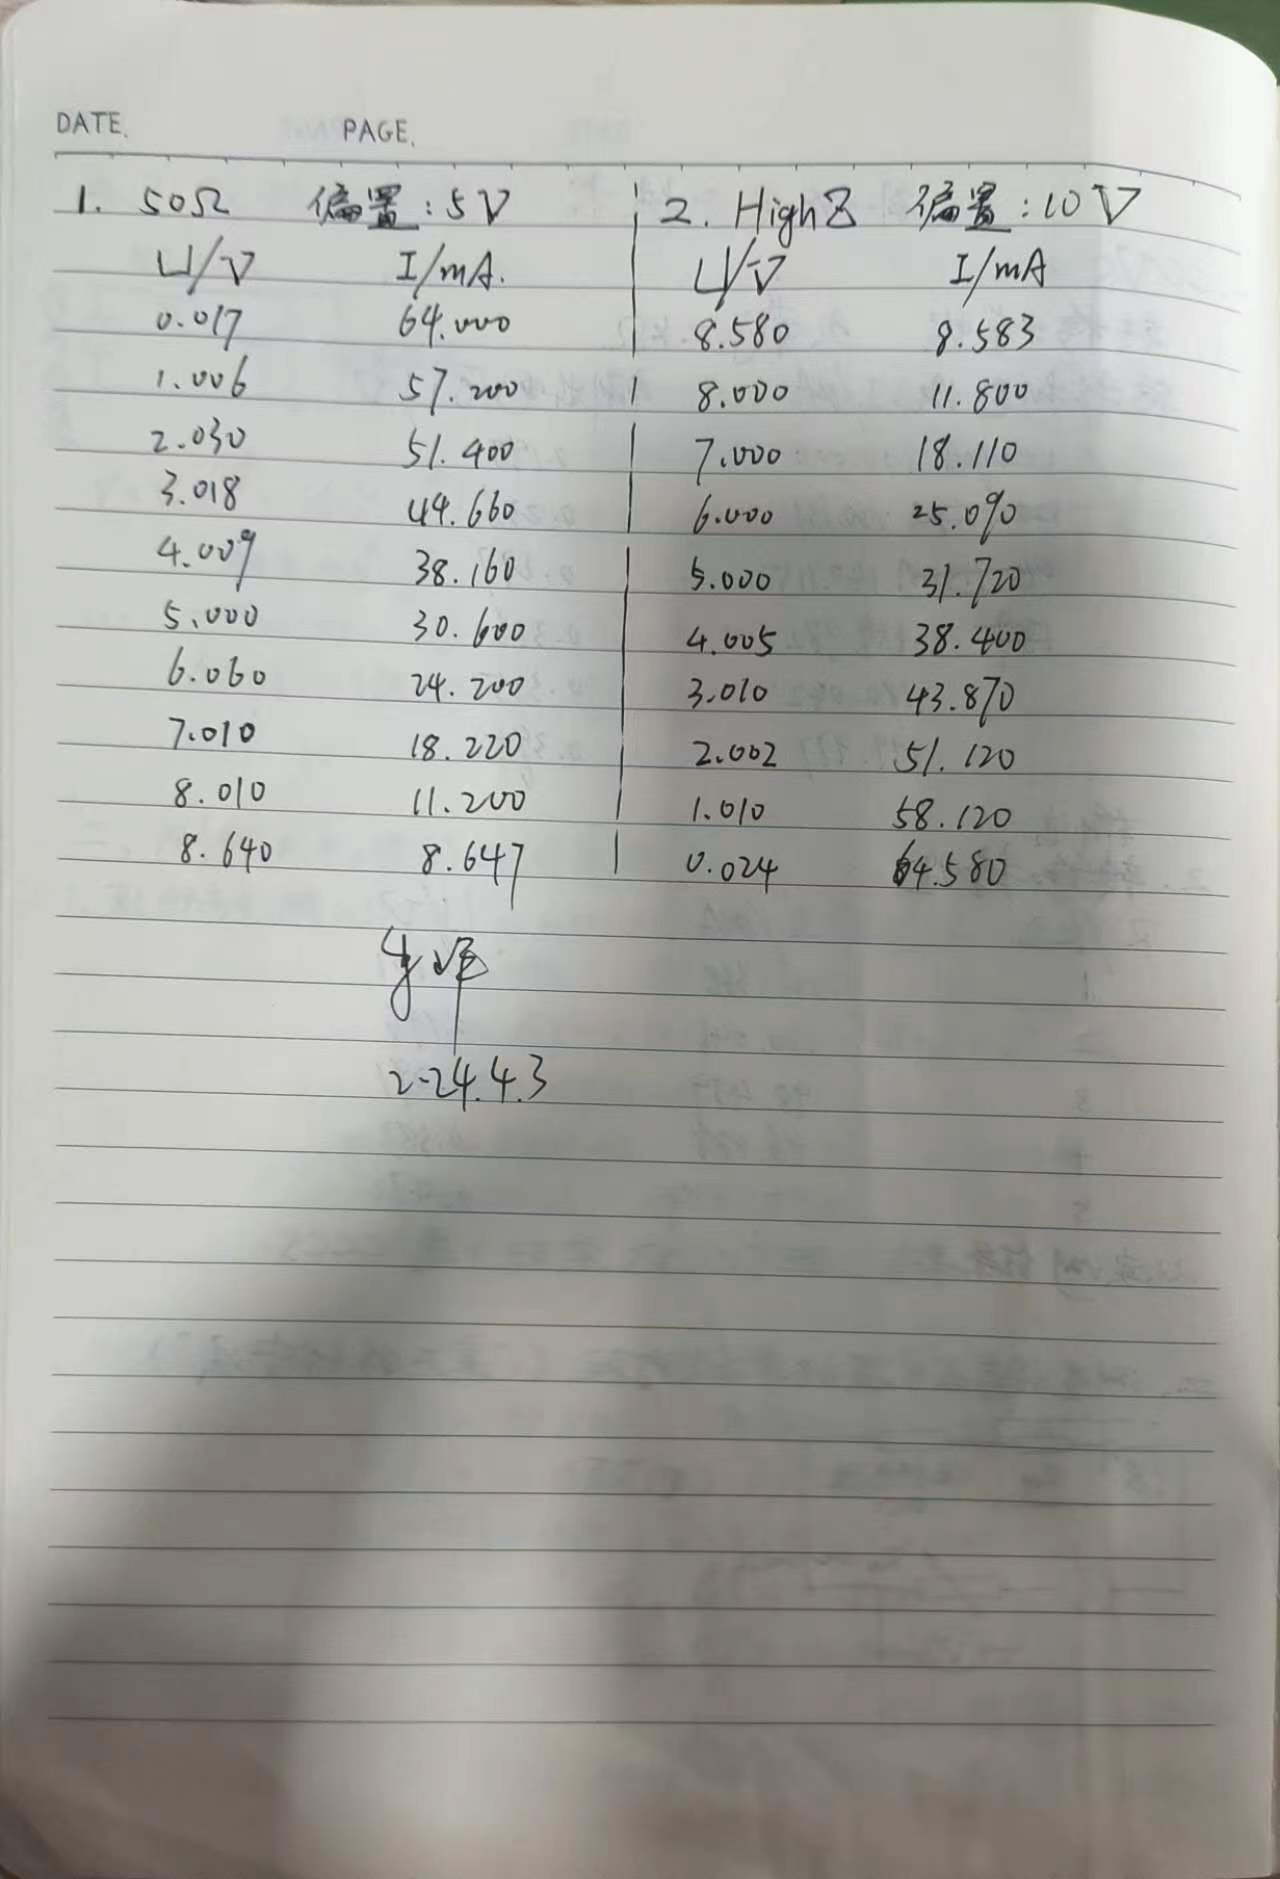
\includegraphics[width=0.28\textwidth]{ET1_4Gradata-6.jpg}\label{fig:figdata-6}}
		\quad
		\caption{实验原始数据}
		\label{fig:graph10}
	\end{figure}
	
	%实验台桌面整理见%\textbf{附件}部分(\cref{})。
	
	%其它原始数据见%\cref{}。
	% ---
	
	% 问题记录
	\subsection{实验过程遇到问题及解决办法}
	\begin{enumerate}
		\item 在初次进行实验时,我们遇到了函数信号发生器在经过50欧到高阻的切换后实际输出值并不等于设定输出值的问题,给我们造成了巨大的困扰。在老师的协助下,我们对这一问题进行了一定的探究,对函数信号发生器的使用方法更加了解了,并发现了函数信号发生器的一点小Bug。
	\end{enumerate}
	% ---
	
	
	
	% 分析与讨论	
	\clearpage
	
	% 顶栏
	\begin{table}
		\renewcommand\arraystretch{1.7}
		\begin{tabularx}{\textwidth}{|X|X|X|X|}
			\hline
			专业:& 物理学 &年级:& 2022级\\
			\hline
			姓名: & 戴鹏辉、杨舒云 & 学号:& 22344016、22344020\\
			\hline
			日期:& 2024/4/8 & 评分: &\\
			\hline
		\end{tabularx}
	\end{table}
	% ---
	
	% 小标题
	\section{ET1-4 戴维南定理和诺顿定理 \quad\heiti 分析与讨论}
	% ---
	
	% 数据处理
	\subsection{实验数据分析}
	
	%
	\subsubsection{关于实验用有源一端口网络的理论计算与仿真}
	
	实验用有源一端口网络的电路图如\cref{fig:graph2}所示,计算其开路电压可将电路等效为\cref{fig:graph3},计算其等效电阻可将电路等效为\cref{fig:graph4}。

	% \begin{figure}[htbp]
	% 	\centering
	% 	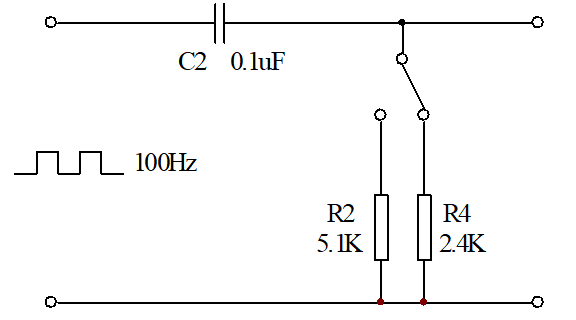
\includegraphics[width=0.6\textwidth]{graph2.png}
	% 	\caption{实验用有源一端口网络}
	% 	\label{fig:graph2}
	% \end{figure}







	
	\begin{enumerate}
		\item 开路电压
		
		\begin{figure}[htbp]
			\centering
			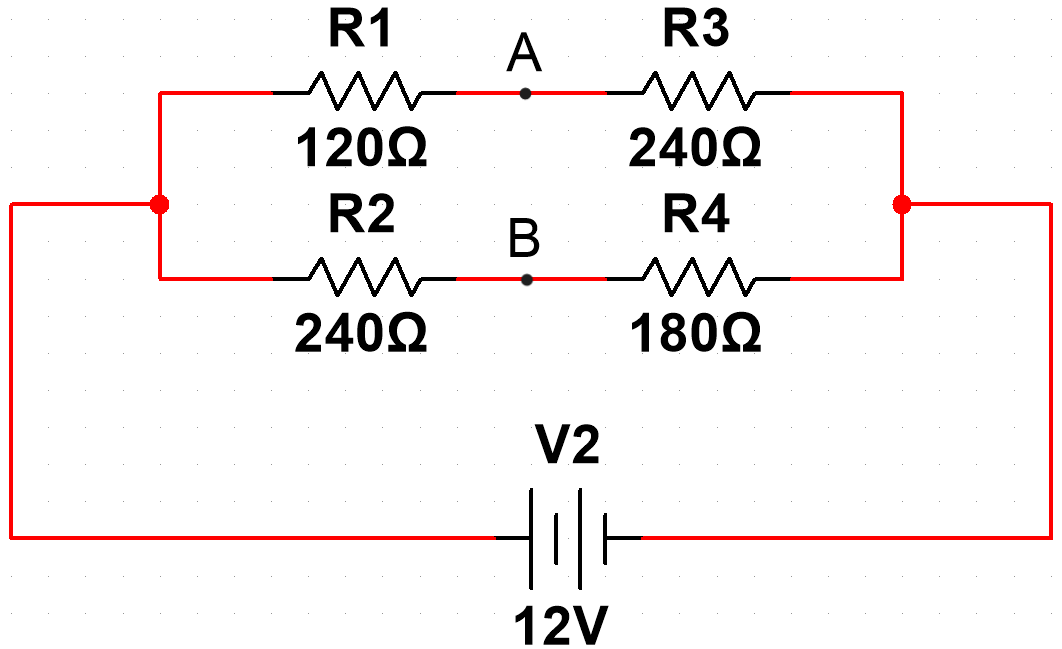
\includegraphics[width=0.4\textwidth]{graph3.png}
			\caption{实验用有源一端口网络简化图}
			\label{fig:graph3}
		\end{figure}

		根据等效电路图\cref{fig:graph3},我们考虑外加一个电压$U$,利用电势降落法分别计算A、B两点的电势,它们之间的电势差即开路电压$U_{OC}=4V$。
		
		\item 等效电阻
		
		\begin{figure}[htbp]
			\centering
			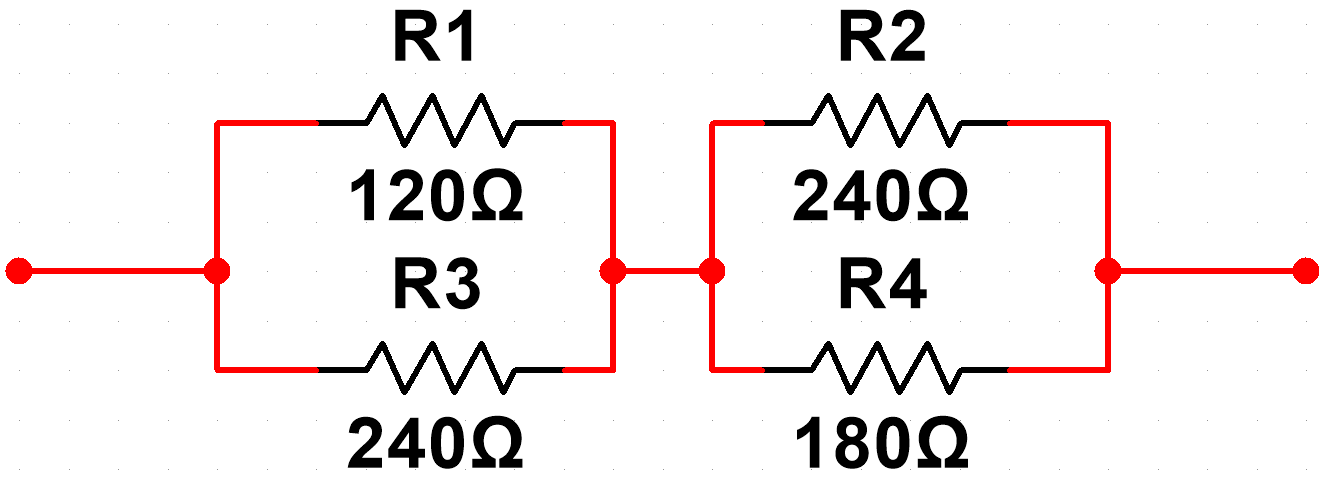
\includegraphics[width=0.4\textwidth]{graph4.png}
			\caption{实验用有源一端口网络电阻简化图}
			\label{fig:graph4}
		\end{figure}

		根据等效电路图\cref{fig:graph4},我们可以直接计算得到等效电阻$R_{eq}=200\Omega$。
		
		\item 短路电流
		
		短路电流$I_{SC}=\dfrac{U_{OC}}{R_{eq}}=0.02A$。
	\end{enumerate}
	
	%
	\subsubsection{误差分析}
	\begin{enumerate}
		\item 对比上一小节计算得到的理论值,结合实验测定的数据,
			我们可以计算出用各种方法测得的各测量量的误差情况,如表所示。



			\begin{table}[htbp]
				\centering
				\begin{tblr}{
					cells = {c},
					vline{1-2,6} = {-}{},
					hline{1-2,4} = {-}{},
				}
					& 理论计算 & 直接测量   & 电压零示法  & 电流零示法  \\
					$U_{OC}/V$ & 4.000    & 3.965  & 3.914  & 3.913  \\
					相对误差  &      & 0.88\% & 2.15\% & 2.18\% 
				\end{tblr}
				\caption{测量有源一端口网络开路电压实验数据}
				\label{tbl:data1}
				
			\end{table}



			\begin{table}[htbp]
				\centering
				\begin{tblr}{
				cells = {c},
				vline{1-2,9} = {-}{},
				hline{1-2,4} = {-}{},
				}
							& 理论计算 & 开路电压、短路电流法 & 伏安法1   & 伏安法2   & 半流法    & 半压法    & 姆表直接测量 \\
					$R_{eq}/\Omega$  & 200  & 199.246    & 196.46 & 196.62 & 193    & 193.5  & 200.1  \\
					相对误差 &      & 0.38\%     & 1.77\% & 1.69\% & 3.50\% & 3.25\% & 0.05\% 
				\end{tblr}
				\caption{测量有源一端口网络等效电阻实验数据}
				\label{tbl:data2}
			\end{table}


			% \begin{table}
			% 	\centering
			% 	\begin{tblr}{
			% 	cells = {c},
			% 	vline{1-2,5} = {-}{},
			% 	hline{1-2,4} = {-}{},
			% 	}
			% 		& 线性网络供电 & 外置电压源供电 & 外置电流源供电 \\
			% 	$U_{R_6}/V$ & 1.315  & 1.296   & 1.250   \\
			% 	$I_{R_6}/mA$ & 13.302 & 13.050  & 12.900  
			% 	\end{tblr}
			% 	\caption{验证戴维南定理和诺顿定理实验数据}
			% \end{table}

			\begin{table}[htbp]
				\centering
				\begin{tblr}{
				  column{even} = {c},
				  column{1} = {c},
				  column{3} = {c},
				  vline{1-2,6} = {-}{},
				  hline{1-2,4} = {-}{},
				}
					& 线性网络供电 & 外置电压源供电 & 外置电流源供电 & 理论值    \\
					$U_{R_6}/V$ & 1.315  & 1.296   & 1.250   & 1.333  \\
					$I_{R_6}/mA$ & 13.302 & 13.050  & 12.900  & 13.333 
				\end{tblr}
				\caption{验证戴维南定理和诺顿定理实验数据}
				\label{tbl:data3}
				\end{table}

		\item 根据上表\cref{tbl:data1}数据可知,在测量开路电压的实验中,相对误差均在2\%左右,实验精度较高。但所有的实验方法测得的结果均偏小,可能是以下原因导致的:
			\begin{enumerate}
				\item 测量仪器的内阻:如果使用的电压表内阻不够大,可能会对网络造成负载效应,从而降低测量到的电压值。
				\item 接触电阻:测量点之间的接触不良可能导致额外的电阻,影响测量精度。
				\item 电源不稳定:电源供应的不稳定可能导致测量时电压波动,影响结果。
			\end{enumerate}
			
			在测量等效电阻的实验中,根据上表\cref{tbl:data2},开路电压、短路电流法的实验相对误差在0.38\%左右,伏安法的实验相对误差在1.7\%左右,半流法、半压法在3.3\%左右,而使用欧姆表直接测量的实验相对误差在0.05\%,是实验精度最高的方法。实验误差可能的产生原因有:
				\begin{enumerate}
					\item 电阻原因:线路电阻、连接线电阻可能不可忽略,或者电流检测孔接触不完全,这些都会导致测量值偏小。
					\item 电源内阻影响:实际的电压源具有一定内阻,这可能会影响测量精度。
					\item 测量方法的局限性:半电压法和半流法在操作上可能难以精确控制,从而影响结果。
				\end{enumerate}

			在验证戴维南定理和诺顿定理实验中,根据上表\cref{tbl:data3}数据,对比三种供电方式,发现三种方式数据接近,可认为成功验证了戴维南定理和诺顿定理。但是对比理论之后发现,所测得的数据均偏小。可能是因为电表和电源均有内阻,使得电路总内阻增大,使得测得的数据偏小。
			
		% \item (分析产生上述误差的原因)
	\end{enumerate}
	
	%
	\subsubsection{其它问题的进一步讨论与分析}
	\begin{enumerate}
		\item “测电源伏安法”的应用
		\begin{enumerate}
			\item 电源外特性曲线

				电源的外特性曲线是指在不同负载条件下,电源输出端电压与输出电流之间的关系。这条曲线可以帮助我们理解电源在实际使用中的表现,特别是在负载变化时电源的响应。

				一般来说,电源的外特性曲线有以下几个重要特点:
				\begin{enumerate}
					\item 空载电压:当输出电流为零时,电源端的电压称为空载电压。这是外特性曲线与纵轴交点的电压值。
					\item 内阻:电源的内阻是影响外特性曲线形状的一个重要因素。理想电压源的内阻为零,理想电流源的内阻为无穷大。实际电源的内阻介于两者之间,导致输出电压随负载电流增加而降低。
					\item 电压降:当负载电流增加时,电源端电压会因内阻而降低,这个现象称为电压降。

				\end{enumerate}
				
				在绘制外特性曲线时,通常将输出电流$I$作为横轴,输出电压$U$作为纵轴。
			\item 伏安法测量直流电源外特性曲线原理与流程

			
			伏安法是一种常用于测量直流电源外特性曲线的方法。这种方法的基本原理是通过改变负载电阻(或使用一个可变负载)来调节从电源抽取的电流,同时测量电源的输出电压和通过负载的电流,从而获得一系列电压-电流对应点。通过这些数据点,可以绘制出电源的外特性曲线,即输出电压$V$与输出电流$I$之间的关系图。
			
			\textbf{测量原理}:
			
			伏安法的核心在于欧姆定律$V = IR$,即电压$V$等于电流$I$乘以电阻$R$。通过改变电阻$R$的值,我们可以得到不同的电流$I$和电压$V$读数,这些读数反映了电源在不同负载条件下的表现。对于直流电源,理想的外特性曲线是一条水平线,表示输出电压不随输出电流的变化而变化。然而,实际的曲线通常会有所下降,这是因为电源内部的电阻和其他因素导致的电压降。
			
			% \textbf{测量流程}:
			% \begin{enumerate}
			% 	\item 准备工具与设备:需要直流电源、可变负载(如可变电阻器或电子负载)、电压表和电流表。如果电压表和电流表是数字式的,可以提供更高的测量精度。
			% 	\item 连接电路:将电压表并联在电源输出端,以测量输出电压;将电流表串联在电路中,以测量流经负载的电流。确保所有连接正确无误,避免短路。
			% 	\item 测量与记录:从最小负载(最高阻值)开始,逐渐减小电阻值(增大负载),在每个设定的负载下记录电源的输出电压和电流。重要的是要平稳且缓慢地调整负载,以避免电源或负载因快速变化而受损。
			% 	\item 绘制曲线:使用测量得到的电压-电流对应点,在坐标纸或使用图表软件绘制外特性曲线。横轴通常表示输出电流$I$,纵轴表示输出电压$V$。
			% 	\item 分析与评估:通过分析外特性曲线,可以评估电源的性能,如稳定性、负载调节率和线性度。理想情况下,曲线应尽可能接近水平,表示电源能够在不同负载下保持稳定的输出电压。
			% \end{enumerate}


			\item 利用“测电源的伏安法”测量函数信号发生器的电动势与等效内阻
			
			按照\textbf{实验步骤}当中的叙述和\textbf{实验结果}所记录的数据,我们可以绘制图像如\cref{fig:graph6}所示:
			
			\begin{figure}[htbp]
				\centering
				\subfloat[$50\Omega$模式]
				{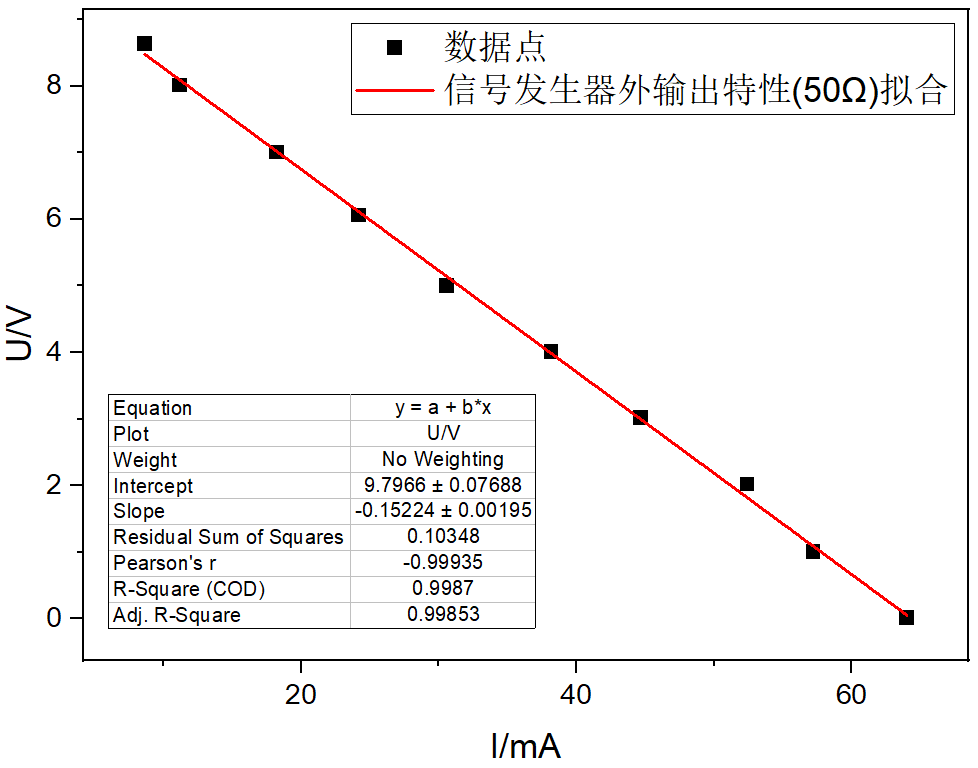
\includegraphics[width=0.45\textwidth]{graph6-50omega.png}\label{fig:graph6-50omega}}
				\quad
				\subfloat[$HighZ$模式]
				{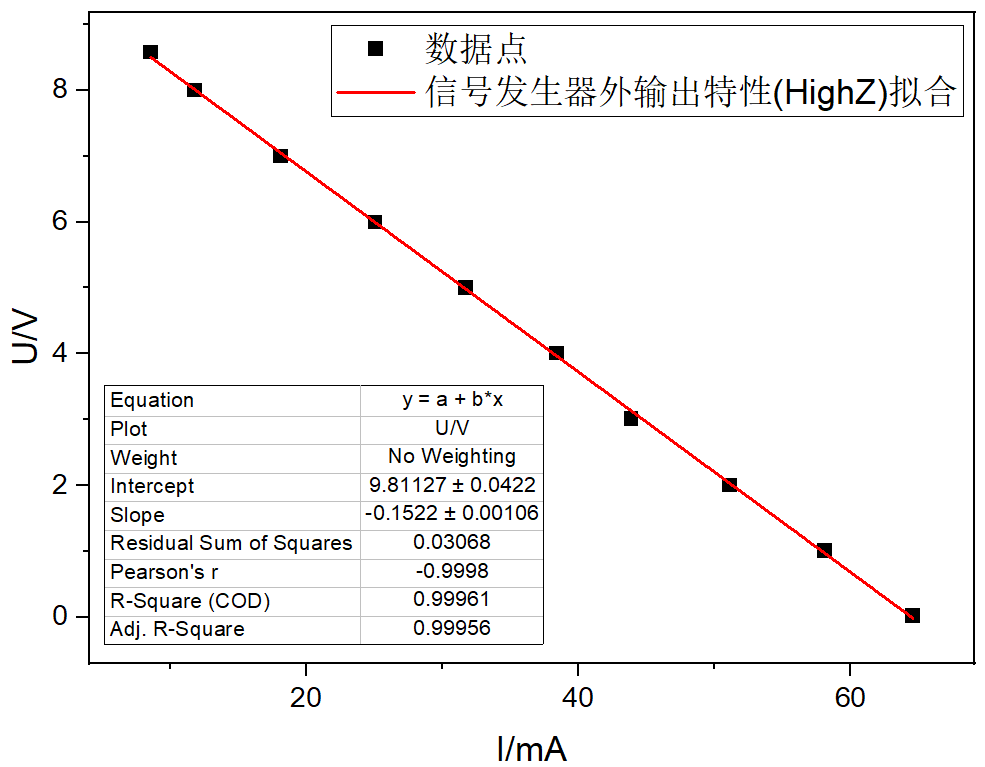
\includegraphics[width=0.45\textwidth]{graph6-HighZ.png}\label{fig:graph2-42}}
				\quad
				\caption{信号发生器外输出特性曲线}
				\label{fig:graph6}
			\end{figure}
			
			从图中可以读出,$50\Omega$模式时,纵轴截距读出输出电压为9.80V,斜率读出等效内阻为152$\Omega$;$HighZ$模式时,纵轴截距读出输出电压为9.81V,斜率读出等效内阻为152$\Omega$。可见,不论信号发生器选择$50\Omega$模式或$HighZ$模式,所测得的信号发生器输出电压都接近设定的10V,内阻也均是50$\Omega$.
			
			
			\item 伏安法测量直流电源外特性曲线误差
			
				使用伏安法测量电源外特性曲线时,也会引入一定的误差,如:
				\begin{enumerate}
					\item 电表内阻引起的误差:在伏安法测量中,电压表和电流表的内阻会对测量结果产生影响。如果电压表的内阻不是很大,那么它会与电源并联,从而引起分流效应,导致测量的电流值偏小。同样,如果电流表的内阻不是很小,它会与负载串联,引起分压效应,导致测量的电压值偏小。
					\item 电源的稳定性:如果电源在测量过程中不够稳定,其电动势和内阻的变化也会引起测量误差。
				\end{enumerate}
				
		\end{enumerate}
		\item 关于函数信号发生器的等效内阻的的进一步讨论与分析
		
		
		函数信号发生器是一种广泛应用于电子实验、电路测试和信号处理等领域的电子设备,它能产生具有特定形状(如正弦波、方波、三角波等)、频率和幅度的电信号。函数信号发生器的等效内阻(也称为输出阻抗)是一个重要的参数,它影响信号发生器与外部负载连接时的信号传输和负载性能。
		
		\textbf{等效内阻的基本概念}:
		
		等效内阻是指信号源内部由于各种原因产生的电阻效应,这个参数对于信号的输出能力有着直接的影响。在理想情况下,信号发生器的等效内阻应当是0欧姆,这意味着信号发生器能够无损耗地将信号完全传递给负载。然而,在实际应用中,任何电子设备都会有一定的内阻,这就会导致输出信号在传递过程中发生衰减。
		
		\textbf{信号发生器的高阻特性}:
		
		高阻输出是函数信号发生器的一种常见特性,通常意味着输出阻抗在几千欧姆到数万欧姆范围内。高阻输出的主要优点是能够最小化因负载变化引起的信号幅度变化,这对于确保输出信号的稳定性和精确性至关重要。
		
		\begin{enumerate}
			\item 信号稳定性:高阻输出可以使信号发生器与各种负载连接时,其输出信号的稳定性不受负载阻抗变化的影响,特别是在负载阻抗远大于信号发生器内阻的情况下。
			\item 最小负载影响:由于高阻能够减少电流的流出,因此能够减轻负载对信号源本身电压的影响,从而保持信号幅度和形状的一致性。
			\item 适应性强:高阻输出使得信号发生器能够适应各种不同阻抗的负载,增加了其适用范围。
		\end{enumerate}

		\textbf{高阻的局限性}:
		
		尽管高阻输出有其优点,但也存在一些局限性。例如,高输出阻抗可能导致信号在长距离传输时的衰减增加,尤其是在高频应用中。此外,高阻输出可能不适用于需要低输出阻抗来驱动的负载,如某些类型的放大器输入。
		
		\textbf{应用中的考量}:
		
		在选择和使用函数信号发生器时,需要根据具体的应用需求来考虑其等效内阻的特性。如果应用中负载阻抗较高,或者对信号稳定性的要求极高,那么高阻输出的信号发生器可能是较好的选择。然而,如果应用需要信号通过较长的传输线,或者需要驱动低阻抗的负载,可能就需要考虑使用等效内阻较低的信号发生器或采用外部缓冲器来降低输出阻抗。
		
		总的来说,函数信号发生器的等效内阻是一个重要但需要根据具体情况灵活考虑的参数。了解和正确处理信号发生器的等效内阻,对于确保电子测试和信号处理应用的成功至关重要。
		
	\end{enumerate}
	
	% ---
	
	% 实验后思考题
	%\subsection{实验后思考题}
	
	
	
	% ---
	
	
	% 结语部分
	\clearpage
	
	% 小标题
	\section{ET1-4 戴维南定理和诺顿定理 \quad\heiti 结语}
	% ---
	
	% 总结、杂谈与致谢
	\subsection{实验心得和体会、意见建议等}
	\begin{enumerate}
		\item 实验心得体会
		\begin{enumerate}
			\item 加深理解:通过本次实验,对戴维南定理和诺顿定理的理解更加深入,能够将理论知识与实践操作相结合,感受到了理论知识在实际电路设计中的应用价值。
			
			\item 操作技能的提升:实验中对电路的搭建、测量仪器的使用等操作更加熟练,特别是在使用万用表、稳压源等设备进行电压和电流的测量时,能够更准确地获取数据。
			
			\item 问题解决能力的增强:面对实验过程中遇到的问题,如函数信号发生器输出值不等于设定值的问题,通过老师指导和自我探索,最终找到了问题的原因并解决了问题。这不仅提高了实验技能,也增强了解决问题的能力。
			
			\item 团队协作:实验的完成是团队合作的结果。在实验过程中,通过与队友的沟通协作,共同讨论问题,相互学习,使得实验工作更加高效,也增强了团队合作意识。
		\end{enumerate}
		
		\item 意见和建议
			\begin{enumerate}
				\item 实验指导书的改进:建议对实验指导书进行一些修改,特别是在实验步骤的描述上,能够更加详细一些,对于实验中可能遇到的常见问题给出提示或解决方案,以帮助学生更好地完成实验。
				
				\item 实验设备的维护:实验中遇到的一些设备问题,如函数信号发生器的小Bug,虽然最终得以解决,但建议定期对实验设备进行检修和维护,确保实验的顺利进行。
				
				\item 增加实验课时:考虑到实验内容的丰富性和实验操作的复杂度,建议增加实验课时,以便学生有足够的时间深入理解实验原理,完成实验操作。
				
				\item 鼓励创新实验:除了完成规定的实验项目外,鼓励学生尝试将所学知识应用到新的实验设计中,发挥创新思维,设计出具有一定创新性的电路,进一步提高实践能力和创新能力。
			\end{enumerate}
			
		\item 感谢老师能阅读这篇还有很多不足的实验报告,希望老师能指出做得不好的地方;祝老师身体健康、生活幸福、工作顺利!
	\end{enumerate}
	% ---
	
	% 参考文献
	\subsection{参考文献}
	[1] 维基百科 https://zh.wikipedia.org
	
	[2] 电子技术实验 保延翔 2020.07 中山大学公共实验教学中心
	
	% ---
	
	% 附件
	\subsection{附件及实验相关的软硬件资料等}
	试验台桌面整理如\cref{fig:table}所示。

	\begin{figure}[htbp]
		\centering
		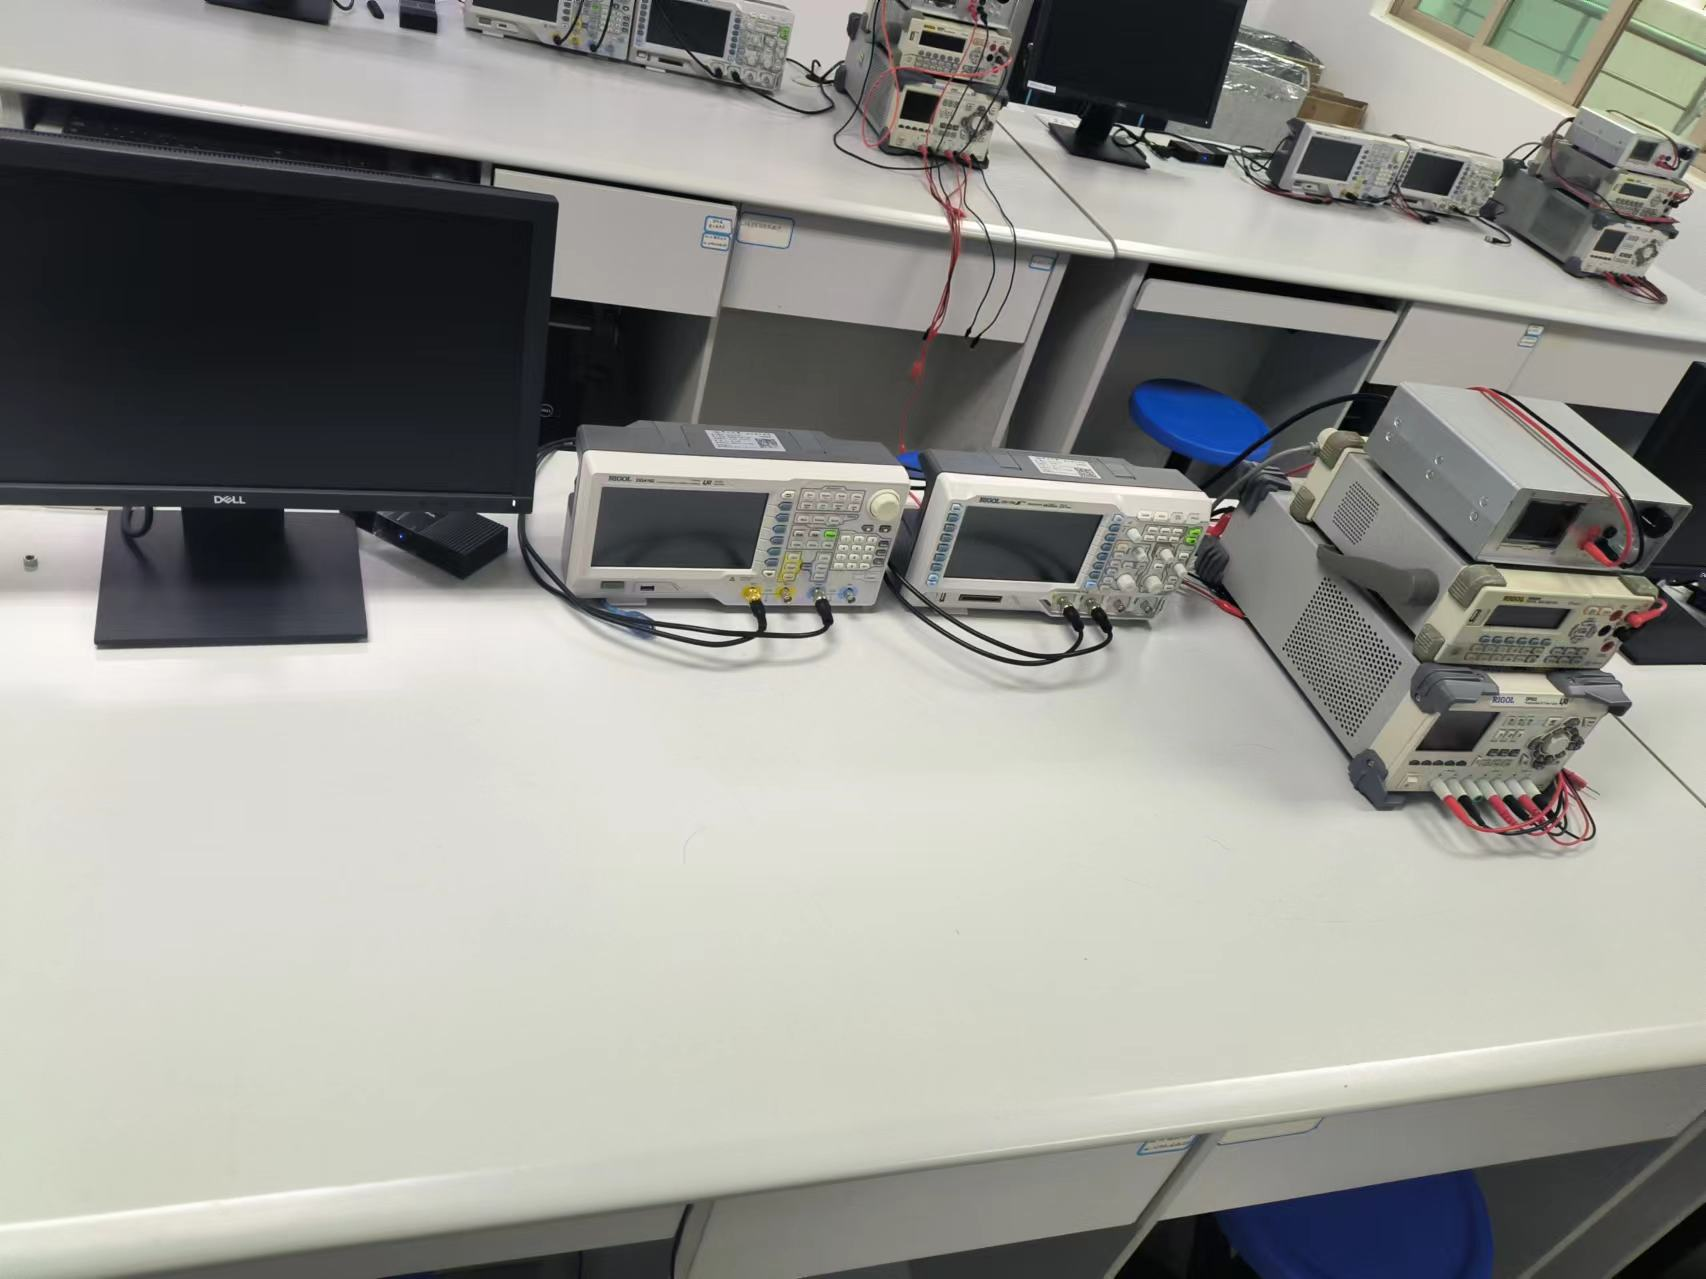
\includegraphics[width=0.5\textwidth]{table.jpg}
		\caption{试验台桌面整理}
		\label{fig:table}
	\end{figure}
	
	实验报告个人签名如\cref{fig:name}。
	
	\begin{figure}[htbp]
		\centering
		\subfloat[]{
			
\includegraphics[width=0.45\textwidth]{name.png}
		}
		\subfloat[]{
			
\includegraphics[width=0.45\textwidth]{name-TaLEs.jpg}
		}
		\caption{个人签名}
		\label{fig:name}			
	\end{figure}
	
	% ---
	
	相关代码已上传至Github。
	
	
	
\end{document}